% !TeX encoding = UTF-8
% !TeX spellcheck = es_ES
\documentclass[12pt]{article}
\usepackage{fullpage}
\usepackage[utf8]{inputenc}
\usepackage{pict2e}
\usepackage{amsmath}
\usepackage{enumitem}
\usepackage{eurosym}
\usepackage{mathtools}
\usepackage{amssymb, amsfonts, latexsym, cancel}
\setlength{\parskip}{0.3cm}
\usepackage{graphicx}
\usepackage{fontenc}
\usepackage{setspace}
\usepackage{adjustbox}
\setstretch{1.35}
\usepackage{bold-extra}
\usepackage{subcaption}
\graphicspath{ {images/} }
\usepackage{tcolorbox}
\usepackage{xcolor, colortbl}
\usepackage{wrapfig}
\usepackage{empheq}
\usepackage{array}
\usepackage{parskip}
\usepackage{arydshln}
\renewcommand*\contentsname{\color{black}Índice} 
\usepackage{array, multirow, multicol}
\definecolor{lightblue}{HTML}{007AFF}
\usepackage{color}
\usepackage{etoolbox}
\usepackage{listings}
\usepackage{mdframed}
\setlength{\parindent}{0pt}
\usepackage{underscore}
\usepackage{hyperref}
\usepackage{tikz}
\usetikzlibrary{shapes, positioning, patterns}
\usepackage{tikz-qtree}
\usepackage{biblatex}
\usepackage{pdfpages}
\usepackage{pgfplots}
\usepackage{pgfkeys}
\usepackage{mathrsfs}
\addbibresource{biblatex-examples.bib}
\usepackage[a4paper, left=1cm, right=1cm, top=1cm,
bottom=1.5cm]{geometry}
\everymath{\displaystyle}
\usetikzlibrary{decorations.pathreplacing}
\usepackage{titlesec}
\setlength{\fboxrule}{1.5pt}
\renewcommand{\arraystretch}{1.2}
\title{Cálculo I}
\author{Francisco Javier Mercader Martínez}
\date{}

% Configura el formato de las secciones utilizando titlesec
\titleformat{\section}
{\color{red}\normalfont\LARGE\bfseries}
{Tema \thesection:}
{10 pt}
{}

% Ajusta el formato de las entradas de la tabla de contenidos
\addtocontents{toc}{\protect\setcounter{tocdepth}{4}}
\addtocontents{toc}{\color{black}}

\titleformat{\subsection}
{\normalfont\Large\bfseries\color{red}}{\thesubsection)}{1em}{\color{lightblue}}

\titleformat{\subsubsection}
{\normalfont\large\bfseries\color{red}}{\thesubsubsection)}{1em}{\color{lightblue}}

\newcommand{\bboxed}[1]{\fcolorbox{lightblue}{lightblue!10}{$#1$}}

\newcommand{\bu}[1]{\textcolor{lightblue}{\underline{#1}}}
\newcommand{\lb}[1]{\textcolor{lightblue}{#1}}
\newcommand{\db}[1]{\textcolor{blue}{#1}}

\newcommand{\dx}{\:\mathrm{d}x}
\newcommand{\dt}{\:\mathrm{d}t}
\newcommand{\dy}{\:\mathrm{d}y}
\newcommand{\dz}{\:\mathrm{d}z}
\newcommand{\dth}{\:\mathrm{d}\theta}
\newcommand{\dr}{\:\mathrm{d}\rho}
\newcommand{\du}{\:\mathrm{d}u}
\newcommand{\dv}{\:\mathrm{d}v}
\newcommand{\tozero}[1]{\cancelto{0}{#1}}
\newcommand{\lbb}[2]{\textcolor{lightblue}{\underbracket[1pt]{\textcolor{black}{#1}}_{#2}}}
\newcommand{\dbb}[2]{\textcolor{blue}{\underbracket[1pt]{\textcolor{black}{#1}}_{#2}}}
\DeclareMathOperator{\N}{\mathbb{N}}
\DeclareMathOperator{\Z}{\mathbb{Z}}
\DeclareMathOperator{\R}{\mathbb{R}}
\DeclareMathOperator{\Q}{\mathbb{Q}}
\DeclareMathOperator{\K}{\mathbb{K}}

\renewcommand{\CancelColor}{\color{lightblue}}
\begin{document}
\maketitle
{\setstretch{1.45} \tableofcontents}
\newpage
\section{Los números naturales}

\subsection{Los números naturales}

Hemos trabajado con ellos desde que apenas tenemos memoria. Hemos aprendido a contar \[ 1,2,3,4,\hdots,n,\hdots\]
Con un orden, \[ 1<2<3<\cdots<n-1<n<n+1 \]
Denotaremos dicho conjunto como $\mathbb{N}$
\begin{itemize}[label=\color{red}\textbullet, leftmargin=*]
	\item \color{lightblue} Propiedades
\end{itemize}
\begin{enumerate}[label=\arabic*)]
	\item Es infinito. Su cardinal es el infinito "más pequeño". Un conjunto para el que existe una biyección con el de los números naturales recibe el nombre de \textit{conjunto numerable}.
	\item Todo subconjunto de $\mathbb{N}$ tiene un elemento mínimo. En esta propiedad se basa el "Principio de Inducción".
\end{enumerate}
Vamos a empezar realizando alguna pequeña demostración utilizando el principio de inducción.
\subsubsection{El Principio de Inducción}
\begin{itemize}[label=\color{red}\textbullet, leftmargin=*]
	\item \color{lightblue} Proposición
\end{itemize}
Supongamos que de una determinada propiedad $P(n)$, en la cual interviene un número natural genérico $n$, si:
\begin{enumerate}[label=\arabic*)]
	\item La propiedad es cierta para $n=1$.
	\item Se supone que la propiedad es cierta para un número $n$ (hipótesis de inducción) se deduce que la propiedad es cierta para $n+1$.
\end{enumerate}
Entonces la propiedad $P(n)$ es cierta para todo número natural $n$.

\begin{itemize}[label=\color{red}\textbullet, leftmargin=*]
	\item \color{lightblue} Ejercicio
\end{itemize}
Establecer la igualdad \[ 1+2+3+\cdots+n=\dfrac{n(n+1)}{2} \]
Para $n\ge 1$ (también lo podemos indicar de la forma $n\in\mathbb{N}$).

Establecer la igualdad \[ a+a^2+\cdots+a^n=\dfrac{a-a^{n+1}}{1-a},~a\neq1 \] para $n\ge1$.

Como sabemos, \[ \mathbb{N}\subset\mathbb{Z}\subset\mathbb{Q}\subset\mathbb{R} \]
\subsection{Los números reales}
Los números reales aparecen de forma natural. ¿Cuál es la solución de la ecuación $x^2=2$?

Observa que la solución no puede ser un número racional, ya que si $x=\dfrac{m}{n}$ siendo $m,n\in\mathbb{N}$, en cuyo caso \[ \dfrac{m^2}{n^2}=2, \]\[ m^2=2n^2, \]
Lo cual nos indica que la descomposición factorial del término de la izquierda habrá una potencia par de 2, mientras que en el término de la derecha de la igualdad el número será impar, de donde se sigue que la ecuación no tiene soluciones racionales.

Otro problema, en cuanto a la idea de que algo es necesario si nos quedamos únicamente con los racionales viene dada por el siguiente ejemplo.

Supongamos que $A$ es un conjunto que viene dado por

$A:=\{p\in\mathbb{Q}:p^2<2\}$ y $B$ es el conjunto dado por:

$B=\{p\in\mathbb{Q}:p^2>2\}$. En estos casos es posible demostrar que $A$ no tiene máximo (y $B$ no tiene mínimo), es decir, para cada $p\in A$, existe $q\in A$ tal $p<q$. Veremos las definiciones formales de máximo y mínimo de un conjunto más adelante.

Para demostrar esta afirmación para cada número racional $p>0$ consideramos el número racional $q$ dado de la forma \[ q=p-\dfrac{p^2-2}{p+2}=\dfrac{p^2+2p-p^2+2}{p+2}=\dfrac{2(p+1)}{p+2}. \]
Ahora, \[ q^2-2=\dfrac{4(p+1)^2}{(p+2)^2}-2=\dfrac{4(p^2+1+2p)-2(p^2+4+4p)}{(p+2)^2}=\dfrac{2(p^2-2)}{(p+2)^2}.\]
Si $p\in A$, entonces el numerador de la expresión anterior es negativo, es decir, $p^2-2<0$, y de ahí $q\in A$, pero por otra parte $q>p$ por la propia definición de $q$. Luego para cada $p\in A$ es posible encontrar $q\in A$ tal que $q>p$. La misma demostración se puede aplicar para el caso de $B$.

\subsubsection{Construcción de los números reales}
La construcción de los números reales puede abordarse como una ampliación partiendo de los números naturales, los números racionales y los números negativos (mediante sucesiones de números racionales), no obstante, nosotros utilizaremos la definición axiomática.

\subsection{Definición axiomática de los número reales}
Antes de dar la definición axiomática de los números reales necesitamos precisar algunos conceptos que necesitaremos.
\begin{itemize}[label=\color{red}\textbullet, leftmargin=*]
	\item \color{lightblue} Definición
\end{itemize}
Un cuerpo es una terna $(K,+,\cdot)$ donde $K$ es un conjunto no vacío y $+,\cdot$ son leyes de composición internas en $K$ tales que:
\begin{enumerate}[label=\arabic*)]
	\item $(K,+)$ es un grupo abeliano. Denotaremos por 0 el elemento neutro de $K$ y si $a\in K$ denotaremos por $-a$ al simétrico de $a$.
	\begin{enumerate}[label=\alph*)]
		\item $\cdot$ es asociativa.
		\item  $\cdot$ es conmutativa.
		\item Existe $1\in K\{0\}$ tal que $1\cdot a=a~~\forall a\in K\{0\}$.
		\item $\forall a\in K\{0\}$ existe $a^{-1}\in K\{0\}$ tal que $a^{-1}\cdot a=1$. A $a^{-1}$ le llamaremos el inverso de $a$.
		\item $a\cdot(b+c)=a\cdot b+a\cdot c~~\forall a,b,c\in K$.
	\end{enumerate}
\end{enumerate}
\begin{itemize}[label=\color{red}\textbullet, leftmargin=*]
	\item \color{lightblue} Definición
\end{itemize}
Dado $A$ un conjunto, una relación binaria $\le$ en $A$ se dice que es una relación binaria de orden si verifica:
\begin{enumerate}[label=\arabic*)]
	\item $a\le a~~\forall a\in A$. (Propiedad Reflexiva).
	\item Si $a,b\in A$ tal que $a\le b\wedge b\le a\rightarrow a=b$. (Propiedad Antisimétrica).
	\item Si $a,b,c\in A$ tal que $a\le b\wedge b\le c\rightarrow a\le c$. (Propiedad transitiva).
\end{enumerate}
Un conjunto ordenado es un par $(A,\le)$ donde $A$ es un conjunto y $\le$ es una relación binaria de orden definida en $A$.

\textbf{¿Qué cuerpos conoces?}

Fíjate en el conjunto $A=\{0,1\}$ con las operaciones:
\begin{center}
	\begin{tabular}{|c|c|c|}
		\hline
		+ & 0 & 1 \\
		\hline
		0 & 0 & 1 \\
		\hline
		1 & 1 & 0 \\
		\hline
	\end{tabular}\hspace{3cm}
	\begin{tabular}{|c|c|c|}
		\hline
		* & 0 & 1 \\
		\hline
		0 & 0 & 0 \\
		\hline
		1 & 0 & 1 \\
		\hline
	\end{tabular}
\end{center}
\textbf{¿Es $\mathbb{N}$ un cuerpo? ¿Es $\mathbb{Q}$ un cuerpo?}

Otro concepto a tener en cuenta es el \textbf{"orden"}. Recordaremos algunos conceptos. 

Veamos:
\begin{itemize}[label=\color{red}\textbullet, leftmargin=*]
	\item \color{lightblue} Definición
\end{itemize}
Sea $(A,\le)$ un conjunto ordenado, $B\subseteq A$ y $a\in A$.
\begin{enumerate}[label=\arabic*)]
	\item Diremos que $a$ es cota superior de $B$ si $b\le a$ para cada $b\in B$.
	\item Diremos que $a$ es cota inferior de $B$ si $a\le b$ para cada $b\in B$.
	\item Diremos que $a$ es el supremo de $B$ si:
	\begin{enumerate}[label=\arabic*)]
		\item $a$ es cota superior de $B$.
		\item Si $a'$ es otra cota superior de $B$ entonces $a\le a'$.
	\end{enumerate}
	\item Diremos que $a$ es el ínfimo de $B$ si:
	\begin{enumerate}[label=\arabic*)]
		\item $a$ es cota inferior de $B$.
		\item Si $a'$ es otra cota inferior de $B$ entonces $a'\le a$.
	\end{enumerate}
\end{enumerate}
Sea $A$ un conjunto ordenado, $B\subseteq A$ y $b\in B$.
\begin{enumerate}[label=\arabic*)]
	\item Diremos que $b$ es un elemento maximal (o máximo) de $B$ si no existe $b'\in B$ con $b\le b'$ y $b\neq b'$.
	\item Diremos que $b$ es un elemento minimal (o mínimo) de $B$ si no existe $b'\in B$ con $b'\le b$ y $b\neq b'$.
\end{enumerate}
\begin{itemize}[label=\color{red}\textbullet, leftmargin=*]
	\item \color{lightblue} Definición
\end{itemize} 
Llamaremos \textcolor{lightblue}{conjunto de los números reales} a un conjunto, que representaremos por $\mathbb{R}$, que verifica los siguientes axiomas:
\begin{enumerate}[label=\arabic*)]
	\item El conjunto $\mathbb{R}$ tiene estructura de cuerpo.
	\item En $\mathbb{R}$ hay definida una relación de orden, (es decir, una relación que verifica las propiedades reflexivas, antisimétrica y transitiva) que es total (siempre se verifica $x\le y$ o bien $y\le x$) para cualesquiera $x,y\in\mathbb{R}$ y compatible con la estructura de cuerpo (si $x\le y$ entonces $x+z\le y+z$, y si $z\ge0$, entonces $xz\le yz$).
	\item Existencia de supremo en $\mathbb{R}$. Todo conjunto no vacío de $\mathbb{R}$ acotado superiormente tiene extremo superior (supremo) en $\mathbb{R}$.
\end{enumerate}
El siguiente paso sería asegurarnos de la existencia del conjunto de los números reales, sin embargo, no nos ocuparemos aquí de ese paso. Remitimos al lector a algunas referencias en donde algunas construcciones clásicas como el método de las cortaduras en $\mathbb{Q}$ de Dedekind (1831-1916) y la construcción de Cantor (1845-1918) utilizando sucesiones de Cauchy de números racionales son algunas posibilidades. 

Ver por ejemplo \textit{Constructions of the real numbers}. 

Los elementos de $\mathbb{R}\backslash\mathbb{Q}$ se llaman \textit{irracionales}, y los denotaremos por $\mathbb{I}$. Más adelante hablaremos de ellos y de su cardinal. Habitualmente los números reales se representan por medio de puntos de una recta. Se elige un punto para representar el 0 y otra para representar la unidad 1. Esta elección determina la escala. El orden de los números viene dado por su representación en la recta.
\begin{itemize}[label=\color{red}\textbullet, leftmargin=*]
	\item \color{lightblue} Proposición (Propiedad arquimediana de los números reales)
\end{itemize}
Para cada par de elementos $x,y\in\mathbb{R}$, tal que $x>0$, existe $n\in\mathbb{Z}$ tal que $y<nx$.
\begin{itemize}[label=\color{red}\textbullet, leftmargin=*]
	\item \color{lightblue} Demostración
\end{itemize}
Sea el conjunto $A=\{mx:m\in\mathbb{Z}\}$. Supongamos que la afirmación no fuera cierta, es decir, para todo $n\in\mathbb{Z}$ y $y>mx$, luego el conjunto $A$ está acotado superiormente. Por el axioma del supremos existe $\alpha\in\mathrm{R}$ tal que $\alpha=\mathrm{sup}(A)$. Puesto que $x>0$, tenemos que $\alpha-x<\alpha$, luego existe $s\in\mathbb{Z}$ tal que $\alpha-x<sx$ y así: \[ a<sx+x=(s+1)x, \]lo cual es absurdo puesto que $\alpha$ es el supremo de $A$. De aquí deducimos que la propiedad es cierta. 

Apoyándonos en la propiedad arquimediana podemos afirmar que para cada número real $y\in\mathbb{R}$ y $x\in\mathbb{R}$ y $x>0$, existen $m,n\in\mathbb{Z}$ tales que \[ mx<y<nx \]
Es decir, \[ mx<(m+1)x<\cdots<px<\cdots<(n-1)x<nx \]
Luego existirá un entero $p\in\mathbb{Z}$ tal que \[ (p-1)x\le y<px \]
Tomando $x=1$, podemos entonces asegurar la existencia de un entero $p$ tal que \[ p-1\le y<p \]
\begin{itemize}[label=\color{red}\textbullet, leftmargin=*]
	\item \color{lightblue} Definición
\end{itemize}
Al número $p-1\in\mathbb{Z}$ se le llama parte entera de $y$ y se le denota $E(y)$ o $[y]$.
\subsection{Valor absoluto}
\begin{itemize}[label=\color{red}\textbullet, leftmargin=*]
	\item \color{lightblue}Definición
\end{itemize}
Se llama valor absoluto de $x\in\mathbb{R}$ al número real denotado por $|x|$ dado por \[ |x|=\max\{x,-x\} .\]
Es decir, \[ |x|=\left\lbrace\begin{array}{cl}
	x & \text{si }x\ge0\\
	-x & \text{si }x<0
\end{array}\right. .\]
\subsubsection{Propiedades del valor absoluto}
\begin{itemize}[label=\color{red}\textbullet, leftmargin=*]
	\item \color{lightblue}Proposición
\end{itemize}
\begin{enumerate}[label=\arabic*)]
	\item $|-x|=|x|$.
	\item Para cada $\epsilon>0,~|x|<\epsilon$ es equivalente a $-\epsilon<x<\epsilon$.
	\item $|x|=0$ si y sólo si $x=0$.
	\item $|x+y|\le |x|+|y|$.
	\item $|x-y|\ge|x|-|y|$.
	\item $|x\cdot y|=|x|\cdot|y|$.
	\item $|x^{-1}|=|x|^{-1}$ para cada $x\neq0$.
	\item $\left||x|-|y|\right|\le|x-y|$.
\end{enumerate}
Probaremos únicamente las propiedades \textcolor{lightblue}{(4)} y \textcolor{lightblue}{(5)}:
\begin{enumerate}[label=\arabic*)]
	\item $|x+y|=\max\{x+y,~x-y\}$. Por otro lado $-|x|\le x\le |x|$ y $-|y|\le y\le |y|$, luego $-\left(|x|+|y|\right)\le x+y\le |x|+|y|$ y por la propiedad \textcolor{lightblue}{(2)} tenemos que $|x+y|<|x|+|y|$.
	\item $x=x-y+y$, de donde \[ |x|=\left|(x-y)+y\right|\le|x-y|+|y|, \]de donde, $|x|-|y|\le|x-y|$.
\end{enumerate}
\subsection{Densidad}
\begin{itemize}[label=\color{red}\textbullet, leftmargin=*]
	\item \color{lightblue} Proposición (Densidad de $\mathbb{Q}$ y $\mathbb{I}$)
\end{itemize}
\begin{enumerate}[label=\arabic*)]
	\item Sean $x,y\in\mathbb{R}$ tales que $x<y$. Entonces existe $r\in\mathbb{Q}$ tal que $x<r<y$.
	\item Dados $r,s\in\mathbb{Q}$ tales que $r<s$. Entonces existe $\xi\in\mathbb{I}$ tal que $r<\xi<s$.
\end{enumerate}
Por la propiedad arquimediana, dados $y-x>0$ y $1$, existe $n\in\mathbb{N}$ tal que \[ 1<n(y-x) .\]
Sea $p=E(nx)\in\mathbb{Z}$. Entonces se verifica que $p\le nx<(p+1)$, luego \[ nx<p+1\le nx+1<ny ,\] de donde \[ nx<p+1<ny \] o de forma equivalente \[ x<\dfrac{p+1}{n} <y.\]
Es decir $r=\dfrac{p+1}{n}\in\mathbb{Q}$ verifica la condición buscada. Aplicando a la misma propiedad a $x<r$ podemos afirmar la existencia de $s\in\mathbb{Q}$ tal que $x<s<r$ lo cual muestra  que existen infinitos números racionales cumpliendo la condición del enunciado.

Por otra parte, es posible demostrar que entre dos números racionales $r<s$ existen infinitos irracionales. Sabemos que el número $b\in\mathbb{R}$ tal que $b^2=2$ es irracional y que $b<2$. Entonces, el número $a=\dfrac{b(s-r)}{2}$ es irracional y tenemos que $a<s-r$. Ahora el número $\xi=r+a$ es irracional y $r<\xi<s$.
\subsection{Representación decimal de los números reales}
\begin{itemize}[label=\color{red}\textbullet, leftmargin=*]
	\item \color{lightblue} Definición
\end{itemize}
Se llama números algebraicos a aquellos que son raíces de alguna ecuación polinómica con coeficientes enteros. Los números que no son algebraicos se llaman trascendentes.

Un número real de la forma \[ r=a_0+\dfrac{a_1}{10}+\dfrac{a_2}{100}+\cdots+\dfrac{a_n}{10^n} ,\] donde $a_0$ es un entero no negativo y $a_1,a_2,\hdots,a_n$ son enteros que satisfacen $0\le a_i\le 9$ se escribe de la forma \[ r=a_0,a_1,a_2,\hdots,a_n. \]
En este caso tendríamos una representación decimal finita y el número $r$ es necesariamente racional.

Sin embargo, no todos los números racionales tienen una representación decimal finita. Así, si $\dfrac{1}{3}$ tuviera representación decimal finita tendríamos que $\dfrac{1}{3}=\dfrac{a}{10^n}$ para cierto $a$ y cierto $n$, es decir, $10^n=3a$ lo cual no es posible, puesto que 3 no es divisor de ninguna potencia de 10.

Sin embargo, podemos aproximar cualquier número real $x>0$ por una aproximación decimal con un error tan pequeño como se desee por medio de una suma como la expresada anteriormente basándonos en el hecho de ir dividiendo el intervalo en 10 partes iguales en cada paso de forma que 

\[\begin{array}{rcl}
	a_0&\le x<&a_0+1 \\
	a_0+\dfrac{a_1}{10}&\le x<&a_0+\dfrac{a_1+1}{10}\\
	a_0+\dfrac{a_1}{10}+\dfrac{a_2}{100}+\dfrac{a_2}{100}&\le x<&a_0+\dfrac{a_1}{10}+\dfrac{a_2+1}{100}\\
	&\cdots&
\end{array}\]

Cada número irracional tiene una representación decimal infinita. Observar que es importar tener en cuenta en esta definición dónde situamos la posibilidad de igualdad, ya que utilizando esta situación la representación de $\dfrac{1}{8}$ sería \[ \begin{array}{c}
	0\le\frac{1}{8}<1,\\
	\frac{1}{10}\le \dfrac{1}{8}<\frac{2}{10}\\
	\frac{1}{10}+\frac{2}{100}\le\frac{1}{8}<\frac{1}{10}+\frac{3}{100}\\
	\frac{1}{10}+\frac{2}{100}+\frac{5}{1000}\le\frac{1}{10}+\frac{2}{100}+\frac{6}{1000}
\end{array} \] y la representación de $\frac{1}{8}$ sería $0.125$, sin embargo si colocamos el signo menor estricto en lugar de menor o igual e incluimos la posibilidad de que sea mayor o igual por exceso tendríamos que la representación de $\frac{1}{8}$ sería $ 0.1249999\hdots$  Hemos obtenido de esta forma dos representaciones distintas para el mismo número.

\subsubsection{La representación de los números reales en el ordenador (Python)}
La representación de los números reales en el ordenador. La cantidad de números con los que el ordenador puede trabajar es finita. Esta afirmación debemos tenerla en cuenta cada vez que pensamos en simulaciones pero no sólo eso, también es importante tener en cuenta cómo trabaja y/o almacena en un ordenador un número.
 En Python la clase "float" (64 bits):
 \begin{itemize}
 	\item 1 bit para el signo del número (positivo o negativo).
 	\item  11 bits para el exponente (el rango es $[-1022, 1023]$).
 	\item 53 bits para dígitos significativos.
 \end{itemize}
 \subsection{Cardinal de un conjunto}
 Se llama \textit{cardinal} de un conjunto $A$ al número de elementos de dicho conjunto y se denota $|A|$.
 
 El conjunto vacío, es decir, de cardinal cero se denota por $\varnothing$.
 
 \begin{itemize}[label=\color{red}\textbullet, leftmargin=*]
 	\item \color{lightblue} Definición
 \end{itemize}
 Diremos que un conjunto $B$ es un subconjunto o parte de un subconjunto $A$ o que $B$ está contenido en $A$ si, todos los elementos de $B$ son a su vez elementos de $A$. Es decir, \[ B\subseteq A\longleftrightarrow x\in B\rightarrow x\in A \]
 Un conjunto $A$ de elementos cualesquiera se dice numerable cuando es finito o cuando siendo finito existe una biyección de $A$ sobre el conjunto de los números naturales $\mathbb{N}$.
 \begin{itemize}[label=\color{red}\textbullet, leftmargin=*]
 	\item \color{lightblue}Proposición
 \end{itemize}
 El conjunto de los números racionales, $\mathbb{Q}$, es numerable.
 
 \begin{itemize}[label=\color{red}\textbullet, leftmargin=*]
 	\item \color{lightblue}Demostración
 \end{itemize}
 Sea $Q_k$  el conjunto de todas las fracciones del denominador $k\in\mathbb{N}$. El subconjunto $Q_k^+$ de las que tienen numerador positivo es trivialmente numerable. De igual forma el conjunto $Q_k^-$ de las que tienen numerador negativo también es numerable y así $Q_k=Q_k^-\cup\{0\}\cup Q_k^+$ es numerable. Ahora el conjunto $\mathbb{Q}=\cup_{k\in\mathbb{N}}Q_k$ es numerable.
 
 El cardinal de los números reales recibe el nombre de potencia del uso continuo. Se dice que un conjunto tiene la potencia del conjunto si existe una biyección de dicho conjunto sobre el $\mathbb{R}$. Durante muchos años estuvo planteado (primer problema de Hilbert) el problema de averiguar si existe subconjuntos de $\mathbb{R}$ que no sean numerables ni tengan la potencia del continuo, es decir $|\mathbb{R}|=\aleph_1$. Finalmente se ha demostrado que no se puede dar una respuesta ni afirmativa ni negativa a partir de los axiomas de definición del cuerpo de los números reales. El admitir este supuesto se convierte en una verdadera hipótesis, (hipótesis del continuo).
 \subsection{La idea del infinito}
 Se llama ampliación de $\mathbb{R}$ al conjunto $\overline{\mathbb{R}}=\mathbb{R}\cup\{-\infty,~\infty\}$ y se admite que $-\infty<x<+\infty$ para cada $x\in\mathbb{R}$.
 \begin{itemize}
 	\item $x+(+\infty)=x-(-\infty)=+\infty;~x+(-\infty)=x-(+\infty)=-\infty$.
 	\item Si $x>0,~x\cdot(+\infty)=(+\infty)\cdot x=+\infty$; si $x<0$, entonces $x\cdot(+\infty)=(+\infty)\cdot x=-\infty$.
 	\item Si $x>0,~x\cdot(+\infty)=(-\infty)\cdot x=-\infty$; si $x<0,~x\cdot(-\infty)=(-\infty)\cdot x=+\infty$.
 	\item $\frac{x}{+\infty}=\frac{x}{-\infty}=0$.
 	\item $(+\infty)+(+\infty)=(+\infty)-(-\infty)=(+\infty)\cdot(+\infty)=(-\infty)\cdot(-\infty)=+\infty$.
 	\item $(-\infty)+(-\infty)=(-\infty)-(-\infty)=(-\infty)\cdot(+\infty)=(+\infty)\cdot(-\infty)=-\infty$.
 \end{itemize}
\subsection{Funciones elementales}
\begin{itemize}[label=\color{red}\textbullet, leftmargin=*]
	\item \color{lightblue}Definición
\end{itemize} 
Sea $I\subset\mathbb{R}$. Se llama función real de variable real a toda aplicación $f:I\Rightarrow\mathbb{R}$ tal que $y=f(x)$. $x$ recibe el nombre de variable independiente y el nombre de variable dependiente. Al conjunto $I$ se llama conjunto inicial y al conjunto $\{f(x):x\in I\}$ se le llama conjunto imagen de $I$ mediante $f$. Al conjunto de valores en que la función se encuentra bien definida se le llama dominio de definición de $f$.

Seguimos algunas nociones conocidas:
\begin{itemize}[label=\color{red}\textbullet, leftmargin=*]
	\item \color{lightblue}Definición
\end{itemize}
Una función $f:I\Rightarrow\mathbb{R}$ se dice que es:
\begin{itemize}
	\item  Par si $f(x)=f(-x)$ para cada $x\in I$.
	\item Impar si $f(x)=-f(x)$ para cada $x\in I$.
	\item Creciente si para $x<y$ entonces $f(x)\le f(y)$.
	\item Estrictamente creciente si para $x<y$ entonces $f(x)<f(y)$.
	\item Decreciente si para $x<y$ entonces $f(x)\ge f(y)$.
	\item Estrictamente decreciente si para $x<y$ entonces $f(x)>f(y)$.
\end{itemize}
\subsubsection{Potencias de base real y exponente entero}
\fbox{$f(x)=x^n$}
\begin{itemize}[label=\color{red}\textbullet, leftmargin=*]
	\item \color{lightblue}Proposición (Propiedades)
\end{itemize}
\begin{itemize}
	\item  Si $n>0$ entonces $x^n=x\cdot x\cdot~\cdots~\cdot x$.
	\item Si $n=0,~x^0=1$.
	\item Si $n<0$ entonces $x^n=\dfrac{1}{x^{-n}}$.
	\item $(xy)^n=x^n\cdot y^n$.
	\item $x^n\cdot x^m=x^{n+m}$.
	\item $ \left(x^n\right)^m=x^{n\cdot m}$.
	\item Si $n>0$, entonces $x^n$ es monótona creciente en $(0,+\infty)$
	\item Si $n<0,~x^n$ es monótona decreciente en $(0,-\infty)$
\end{itemize}
\subsubsection{Función exponencial}
Sea $a>0$, se define la función exponencial $f(x)=a^x$.
\begin{itemize}[label=\color{red}\textbullet, leftmargin=*]
	\item \color{lightblue}Proposición (Propiedades)
\end{itemize}
\begin{itemize}
	\item Si $a=1$, la función es constantemente igual a 1.
	\item $a^{x+y}=a^x\cdot a^y,~a^0=1$.
	\item Si $x<y$ y $0<a<1$, entonces $a^y<a^x$.
	\item Si $a>1,~\lim_{x\to\infty}a^x=+\infty,~\lim_{x\to-\infty}a^x=0$.
	\item Si $0<a<1,~\lim_{x\to\infty}a^x=0,~\lim_{x\to-\infty}a^x=+\infty$.
\end{itemize}
\subsubsection{Función logaritmo}
Sea $a>0~f(x)=\log_a(x)$

De aquí,  $y=\log_a(x)$ sí, y sólo si, $a^y=x$.
\begin{itemize}
	\item $\log_a(xy)=\log_a(x)+\log_a(y)$.
	\item $\log_a1=0$.
	\item $\log_a\left(\dfrac{x}{y}\right)=\log_a(x)-\log_a(y)$.
	\item $\log_a x^n=n\log_a(y)$.
	\item Si $a>1$, y $x<y$ entonces $\log_a(x)<\log_a(y)$.
	\item Si $0<a<1$ y $x<y$ entonces $\log_a(x)>\log_a(y)$.
	\item Si $b>0$, entonces $\log_a(x)=\dfrac{\log_b(x)}{\log_a(a)}$.
\end{itemize}
\subsubsection{Funciones trigonométricas}
\[ \begin{array}{lr}
	\tan(x)=\dfrac{\sin(x)}{\cos(x)} & \cot(x)=\dfrac{\cos(x)}{\sin(x)}\\
	\sec(x)=\dfrac{1}{\cos(x)} & \mathrm{cosec}(x)=\dfrac{1}{\sin(x)}
\end{array} \]
Para considerar la inversa (con la composición) de las funciones trigonométricas debemos tener en cuenta que la función debe ser biyectiva, por ello debemos seleccionar de forma adecuada un intervalo en el que esto suceda.

Por último recordamos las definiciones de las funciones hiperbólicas. \[ \sinh(x)=\dfrac{e^x-e^{-x}}{2}\hspace{1cm}\cosh(x)=\dfrac{e^x+e^{-x}}{2} \] que verifican \[ \cosh^2(x)=1+\sinh^2(x) .\]
Investiga: "Big O notation".

Esta notación se utiliza en computación y matemáticas para describir el crecimiento asintótico de la función, \textit{lo rápido que crece o decrece}. Se emplea la letra \textcolor{lightblue}{O} porque a la tasa de crecimiento de una función se le suele llamar \textcolor{lightblue}{orden} de la función.

En muchos casos necesitaremos analizar el tiempo necesario para ejecutar un algoritmo, en nuestro caso, sería el número de pasos a realizar cuando introducimos \textcolor{lightblue}{$n$} valores. Imaginamos que haciendo el cómputo de operaciones obtenemos que la función que nos informa acerca del número de pasos es $S(n)=n^2+2n+1$. En ese caso diremos que $S$ crece con orden cuadrático o lo que es lo mismo de la forma $O(n^2)$.

Formalmente diremos que dadas dos funciones $f$ y $g$, \[ f(x)=O\left(g(x)\right))\hspace{0.5cm}(x\to\infty), \]si existen constantes $K$ y $c$ tales que \[ |f(x)|\le K |g(x)|, \] para $x>c$. De forma análoga \[ f(x)=O\left(g(x)\right) \hspace{0.5cm}(x\to x_0),\] si existen constantes $K$ y $\epsilon>0$ tales que \[ |f(x)|\le C|g(x)|, \] para $|x-x_0|<\epsilon$.
\subsection{Sucesiones de números reales}
\subsubsection{Topología en $\mathbb{R}$}
\begin{itemize}[label=\color{red}\textbullet, leftmargin=*]
	\item \color{lightblue}Definición
\end{itemize}
Diremos que un conjunto $A\subset\mathbb{R}$ es:
\begin{enumerate}[label=\arabic*)]
	\item Abierto, si para cada $x\in A$ existe $\delta>0$ tal que el intervalo $(x-\delta,~x+\delta)\subset A$.
	\item Cerrado, si $\mathbb{R}\backslash A$ es abierto.
\end{enumerate}
Obviamente los intervalos abiertos son conjuntos abiertos, mientras que los intervalos cerrados son conjuntos cerrados.
\begin{itemize}[label=\color{red}\textbullet, leftmargin=*]
	\item \color{lightblue}Definición
\end{itemize}
Diremos que un punto $a\in\mathbb{R}$ es adherente a un conjunto $A\subset\mathbb{R}$ si para cada entorno abierto $U$ del punto $a$ se verifica que $U\cap A\neq\varnothing$.  Al conjunto de los puntos adherentes se le llama adherencia o clausura del conjunto. Se denota por $\overline{A}$.

Diremos que un punto $a\in\mathbb{R}$ es de acumulación a un conjunto $A\subset\mathbb{R}$ si para cada entorno abierto $U$ del punto $a$ se verifica que $U\backslash\{a\}\cap A\neq\varnothing$. Al conjunto de los puntos de acumulación se le llama conjunto derivado y se denota por $A'$.
\subsubsection{Límite de una sucesión de números reales}
Una sucesión de números reales es un subconjunto de $\mathbb{R}$ ordenado según el orden de los números naturales. Es decir, es una aplicación $s:\mathbb{N}\longrightarrow\mathbb{R}$ que a cada número natural le asigna un número real, así una sucesión vendrá dada por $\{s(n):n\in\mathbb{N}\}\subset\mathbb{R}$.
\begin{itemize}[label=\color{red}\textbullet, leftmargin=*]
	\item \color{lightblue}Definición
\end{itemize}
Se dice que una sucesión $(x_n)_n$ de números reales tiene por límite al número $x\in\mathbb{R}$ cuando para cada número real positivo $\epsilon>0$ existe un número natural $v\in\mathbb{N}$ tal que si $n\ge v$ entonces $|x_n-x|\le\epsilon$.

En ese caso lo denotaremos $\lim_{n\to\infty}x_n=x$. A las sucesiones que tienen límite se les llama sucesiones \textit{convergentes}.
\begin{itemize}[label=\color{red}\textbullet, leftmargin=*]
	\item \color{lightblue} Definición
\end{itemize}
Diremos que una sucesión $(x_n)_n$ tiene límite $+\infty$ si para cada $K\in\mathbb{R}$ existe $n_K\in\mathbb{N}$ tal que si $n\ge n_K$ se tiene que $x_n\ge K$, diremos que la sucesión $(x_n)_n$ tiene límite $-\infty$ y lo denotaremos $\lim_{n\to\infty}x_n=-\infty$ si para cada $K\in\mathbb{R}$ existe $n_K\in\mathbb{R}$ tal que si $n\ge n_K$ entonces $x_n\le K$.

Cuando una sucesión tiene límite infinito diremos que la sucesión es divergente, mientras que aquellas sucesiones que no tienen límite finito ni infinito reciben el nombre de oscilantes.
\subsubsection{Sucesiones convergentes}
Obsérvese que si la sucesión $(x_n)_n$ tiene como límite $x$, la sucesión $(x-x_n)_n$ tiene límite 0. Cuando una sucesión de números reales tiene por límite a 0 se dice que esta sucesión es un infinitésimo, esto lo estudiaremos con más detalle en secciones posteriores.
\begin{itemize}[label=\color{red}\textbullet, leftmargin=*]
	\item \color{lightblue}Proposición
\end{itemize}
Si una sucesión $(x_n)_n$ tiene límite, entonces ese límite es único.
\begin{itemize}[label=\color{red}\textbullet, leftmargin=*]
	\item \color{lightblue}Demostración
\end{itemize}
Supongamos que $\lim_{n\to\infty}x_n=x$ y que $\lim_{n\to\infty}x_n=y$. Entonces para cada $\epsilon>0$ existen $v_1\in\mathbb{N}$ y $v_2\in\mathbb{N}$ tales que \[ |x_n-x|\le\frac{\epsilon}{2}, \text{ para cada }n\ge v_1,\text{ y} \]\[ |x_n-y|\le\frac{\epsilon}{2}, \text{ para cada }n\ge v_2.\]
Ahora, utilizando la desigualdad triangular y tomando $n\ge\max\{v_1,~v_2\}$ tenemos \[ 0\le|x-y|\le|x-x_n|+|x_n-y|\le\frac{\epsilon}{2}+\dfrac{\epsilon}{2}=\epsilon. \]
Y así, $x=y$.
\subsection{Sucesión de Cauchy}
\begin{itemize}[label=\color{red}\textbullet, leftmargin=*]
	\item \color{lightblue}Definición 
\end{itemize}
Diremos que una sucesión $(x_n)_n$ es una sucesión de Cauchy si para todo número real positivo $\epsilon>0$ existe un número natural $v$ tal que si $n\ge v$ y $m\ge v$ entonces \[ |x_n-x_m|\le\epsilon. \]
Un espacio métrico $X$ se dice completo si toda sucesión de Cauchy es convergente.

Puede comprobarse que la suma de dos sucesiones de Cauchy es otra sucesión de Cauchy, el producto de dos sucesiones de Cauchy es otra sucesión de Cauchy y el producto de un escalar por una sucesión de Cauchy es otra sucesión de Cauchy.

La siguiente proposición establece que la condición es equivalente a la convergencia en $\mathbb{R}$.
\begin{itemize}[label=\color{red}\textbullet, leftmargin=*]
	\item \color{lightblue}Proposición
\end{itemize}
Una sucesión de números reales $(x_n)_n$ es convergente si, y sólo si, es de Cauchy.

Como corolario obtenemos 

\begin{itemize}[label=\color{red}\textbullet, leftmargin=*]
	\item \color{lightblue}Corolario
\end{itemize}
Toda sucesión de Cauchy $\mathbb{R}$ está acotada.
\subsection{Sucesión monótona creciente (decreciente)}
Veamos algunos casos en los que podemos afirmar que la sucesión es convergente. Antes necesitamos introducir algunas definiciones más.
\begin{itemize}[label=\color{red}\textbullet, leftmargin=*]
	\item \color{lightblue}Definición
\end{itemize}
Diremos que una sucesión $(x_n)_n$ de número reales está acotada inferiormente si existe $r\in\mathbb{R}$ tal que $r\le x_n$ para cada $n\in\mathbb{N}$. Diremos que $(x_n)_n$ está acotada superiormente si existe $R\in\mathbb{R}$ tal que $x_n\le R$ para cada $n\in\mathbb{N}$. Por último diremos que la sucesión está acotada si está acotada inferior y superiormente.

Diremos que una sucesión de número reales $(x_n)_n$ es creciente (decreciente) si $x_{n+1}\ge x_n(x_{n+1}\le x_n)$ para cada $n\in\mathbb{N}$.
\begin{itemize}[label=\color{red}\textbullet, leftmargin=*]
	\item \color{lightblue}Proposición
\end{itemize}
Sea $(x_n)_n$ una sucesión de números reales. Entonces:
\begin{enumerate}[label=\arabic*)]
	\item Si $(x_n)_n$ es una sucesión decreciente y acotada inferiormente, entonces $(x_n)_n$ es convergente.
	\item Si $(x_n)_n$ es una sucesión creciente y acotada superiormente, entonces $(x_n)_n$ es convergente.
\end{enumerate}
\begin{itemize}[label=\color{red}\textbullet, leftmargin=*]
	\item \color{lightblue}Ejemplo
\end{itemize}
Demostrar que la sucesión $x_n=\sqrt{a+\sqrt{a+\cdots+\sqrt{a}}}$ donde $a>0$ es convergente probando que es creciente y acotada. Halla su límite.

Observamos que $x_{n+1}=\sqrt{a+x_n}$ para $n\ge1$ y $x_1=\sqrt{a}$. También observamos que $x_n\le x_{n+1}$ para cada $n\in\mathbb{N}$ (inducción). Para $n=1$ obtenemos $\sqrt{a}\le\sqrt{a+\sqrt{a}}$ y $\sqrt{a+x_n}\le \sqrt{a+x_{n+1}}=x_{n+2}$ y queda demostrado que la sucesión es creciente. Veamos ahora que está acotada. \[ x_{n+1}=\sqrt{a+x_n}\le\sqrt{a+k}\le k \] De la última desigualdad obtenemos: \[ a+k\le k^2\Longleftrightarrow k^2-k-a\ge0\]
Tras resolver la ecuación $k=\dfrac{1+\sqrt{1+4a}}{2}$. Así, la sucesión $(x_n)_n$ es convergente. Su límite es $I=\dfrac{1+\sqrt{1+4a}}{2}$.
\begin{itemize}[label=\color{red}\textbullet, leftmargin=*]
	\item \color{lightblue}Proposición
\end{itemize}
Sea $(x_n)_n,~(y_n)_n$ y $(z_n)_n$ sucesiones de números reales. Entonces:
\begin{enumerate}[label=\arabic*)]
	\item Si $x_n\le y_n$ para cada $n\ge n_0$ para cierto $n_0\in\mathbb{N}$ y ambas sucesiones son convergentes, entonces \[ \lim_{n\to\infty}x_n\le\lim_{n\to\infty}y_n. \]
	\item Si $x_n\le y_n\le z_n$ para cada $n\ge n_0$ para cierto $n_0\in\mathbb{N}$ y $\lim_{n\to\infty}x_n=\lim_{n\to\infty}z_n$, entonces \[ \lim_{n\to\infty}x_n=\lim_{n\to\infty}y_n=\lim_{n\to\infty}z_n. \]
\end{enumerate}
\subsection{Sucesión contractiva}
\begin{itemize}[label=\color{red}\textbullet, leftmargin=*]
	\item \color{lightblue}Definición
\end{itemize}
Se dice que una transformación es contractiva si existe un número $\lambda$ menor que 1 se satisfaga la relación \[ |F(x)-F(y)|\le\lambda|x-y| \]
Para todos los puntos $x$ e $y$ en el dominio de $F$.

El método de Newton es un ejemplo de procedimiento mediante el cual se calcula una sucesión de puntos empleando una fórmula de recurrencia como la siguiente: \[ x_{n+1}=F(x_n)\hspace{0.5cm}(n\ge0) .\]
El algoritmo definido de este modo se denomina iteración funcional. En el caso del método de Newton, la función $F$ viene dada por: \[ F(x)=x-\dfrac{f(x)}{f'(x)}. \]
En aquellos casos para los que se cumple que la sucesión así obtenida es convergente $\lim_{n\to\infty}x_n=s$ es fácil observar que cuando $F$ es continua se cumple que \[ F(s)=F\left(\lim_{n\to\infty}x_n\right)=\lim_{n\to\infty}F(x_n)=\lim_{n\to\infty}x_{n+1}=s. \]
Tenemos por tanto que $F(s)=s$ y denotaremos a $s$ punto fijo la función $F$.

\begin{itemize}[label=\color{red}\textbullet, leftmargin=*]
	\item \color{lightblue} Proposición
\end{itemize} 
Sea $F:C\to C$ una aplicación contractiva que va de un conjunto cerrado $C$ a un conjunto cerrado. Entonces $F$ tiene un punto fijo $s$. Además toda la sucesión que se obtenga de la forma $x_{n+1}=F(x_n)$ con $x_1\in C$ es convergente a $s$.

\begin{itemize}[label=\color{red}\textbullet, leftmargin=*]
	\item \color{lightblue}Ejemplo
\end{itemize}
Demuestra que la sucesión $(x_n)_n$ definida recursivamente de la forma: \[ \left\{\begin{array}{l}
	x_0=-155\\
	x_{n+1}=3-\dfrac{1}{2}|x_n|
\end{array}\right.\] es convergente. Calcula su límite.

Para demostrar que es convergente veremos que la sucesión es contractiva. $F(x)=3-\dfrac{1}{2}|x|$. \[ |F(x)-F(y)|=\left|3-\dfrac{1}{2}|x|-3+\dfrac{1}{2}|y|\right| =\dfrac{1}{2}\left||y|-|x|\right|\le\dfrac{1}{2}|y-x|.\]
Así, la sucesión $(x_n)_n$ converge al punto fijo de $F,~s$. \[ 3-\dfrac{1}{2}|s|=s \]
Si $s>0$ entonces $3=\dfrac{3}{2}s$ y de aquí $s=2$. Por otra parte si $s<0$ entonces la ecuación no tiene solución. Así concluimos que el límite es 2.
\subsection{Sucesiones equivalentes. Infinitésimos e Infinitos}
\begin{enumerate}[label=\arabic*)]
	\item La suma de dos sucesiones convergentes es otra sucesión convergente \[ \lim_{n\to\infty}(x_n+y_n)=\lim_{n\to\infty}x_n+\lim_{n\to\infty} \]
	\item El producto de dos sucesiones convergentes es otra sucesión convergente \[ \lim_{n\to\infty}(x_n+y_n)=\lim_{n\to\infty}x_n\cdot\lim_{n\to\infty}y_n \]
	\item El producto de un escalar por una sucesión convergente es otra sucesión convergente \[ \lim_{n\to\infty}(\lambda x_n)=\lambda\lim_{n\to\infty}x_n \]
	\item El cociente de dos sucesiones convergentes es otra sucesión convergente, siempre que esté bien definida y el límite de la sucesión del denominador sea distinto de 0. Entonces \[ \lim_{n\to\infty}\dfrac{x_n}{y_n}=\dfrac{\displaystyle\lim_{n\to\infty}x_n}{\displaystyle\lim_{n\to\infty}y_n} .\]
\end{enumerate}
\begin{itemize}[label=\color{red}\textbullet, leftmargin=*]
	\item \color{lightblue}Definición
\end{itemize}
Dadas dos sucesiones $(x_n)_n$ e $(y_n)_n$. Diremos que son equivalentes si $\lim_{n\to\infty}\dfrac{x_n}{y_n}=1$. Se llama infinitésimo a toda sucesión cuyo límite es cero.

Algunos infinitésimos equivalentes son los siguientes, donde $(a_n)_n$ es un infinitésimo:
\begin{enumerate}[label=\arabic*)]
	\item $\log(1+a_n)\equiv a_n$
	\item $\sin(a_n)\equiv a_n$
	\item $\tan(a_n)\equiv a_n$
	\item $\arcsin(a_n)\equiv a_n$
	\item $\arctan(a_n)\equiv a_n$
	\item $1-\cos(a_n)\equiv \dfrac{a_n^2}{2}$
	\item $k^{a_n}-1\equiv a_n\log(k)$
	\item $e^{a_n}-1\equiv a_n$
	\item $(1+a_n)^\alpha-1\equiv\alpha a_n$
\end{enumerate}
\begin{itemize}[label=\color{red}\textbullet, leftmargin=*]
	\item \color{lightblue}Definición
\end{itemize}
Diremos que una sucesión $(x_n)_n $ es un infinito si es divergente, es decir, si su límite es $\infty$.

Algunos infinitos equivalentes son:
\begin{enumerate}[label=\arabic*)]
	\item $a_0n^p+a_1n^{p-1}+\cdots+a_p\hspace{0.5cm}p\in\mathbb{N}$.
	\item $\log(a_0n^p+a_1n^{p-1}+\cdots+a_p)\equiv\log(n^p)$ si $a_0>0$.
	\item $n!\equiv e^{-n}n^n\sqrt{2\pi n}$ (Fórmula de Stirling).
\end{enumerate}
\begin{itemize}[label=\color{red}\textbullet, leftmargin=*]
	\item \color{lightblue}Proposición
\end{itemize}
El límite de una sucesión convergente o divergente no se altera al sustituir uno de los factores o divisores por otro factor o divisor que sea equivalente (infinitésimo) a él.
\begin{itemize}[label=\color{red}\textbullet, leftmargin=*]
	\item \color{lightblue}Ejemplo
\end{itemize}
Hallar: \[ \lim_{n\to\infty}\dfrac{8n^6\log\left(1+\dfrac{1}{2n}\right)\sin^3\left(\dfrac{1}{n}\right)}{(2n^2+5n)\cos\left(\dfrac{2\pi n}{6n+3}\right)}. \]
$\log\left(1+\dfrac{1}{2n}\right)\equiv\dfrac{1}{2n},~\sin^3\left(\dfrac{1}{n}\right)\equiv\dfrac{1}{n^3},~2n^2+5n\equiv2n^2$ y $\cos\left(\dfrac{2\pi n}{6n+3}\right)\equiv\cos\left(\dfrac{2\pi n}{6n}\right)$, por lo que el límite queda de la forma \[ \lim_{n\to\infty}\dfrac{8n^6\dfrac{1}{2n}\cdot\dfrac{1}{n^3}}{2n^2\cos\left(\dfrac{2\pi n}{6n}\right)}=4. \]
\subsection{Criterios de convergencia}
\subsubsection{Límites del número $e$}
La base más frecuentemente utilizada para las funciones exponencial y logarítmica es el llamado número $e$ (en honor a Euler). Los logaritmos en base $e$ reciben el nombre de logaritmos neperianos y se denotan por $\log(x)$ o $\ln(x)$. Nosotros utilizaremos $\log(x)$.

Por otra parte, la sucesión $ (r_n)_n $ es una sucesión de Cauchy que es estrictamente creciente y de ahí convergente a un número al que llamamos $e$ cuyo valor aproximado es $2.71828\hdots$

\begin{itemize}[label=\color{red}\textbullet, leftmargin=*]
	\item \color{lightblue} Proposición
\end{itemize}
La sucesión $\left(1+\dfrac{1}{n}\right)^n$ es monótona acotada, luego convergente. El valor de su límite es el número $e$.
\subsubsection{Criterio de Stolz}
Sean $(x_n)_n $ y $(y_n)_n $ dos sucesiones de número reales con $(y_n)_n $ monótona (creciente o decreciente) que cumplen una de las dos siguientes propiedades:
\begin{enumerate}[label=\arabic*)]
	\item $\lim_{n\to\infty}x_n=\lim_{n\to\infty}y_n=0$
	\item $\lim_{n\to\infty}y_n=0$
\end{enumerate}
Entonces, si existe el límite $\lim_{n\to\infty}\dfrac{x_{n+1}-x_n}{y_{n+1}-y_n}$, también existe el límite $\lim_{n\to\infty}\dfrac{x_n}{y_n}$ y ambos límites coinciden. Esto es válido incluso si el límite es $+\infty$ o $-\infty$.
\subsubsection{Criterio de la media aritmética}
Si $(x_n)_n $ es una sucesión convergente de números reales, la sucesión de sus medidas también converge, y se cumple \[ \lim_{n\to\infty}\dfrac{x_1+\cdots+x_n}{n}=\lim_{n\to\infty}x_n. \]
El recíproco no es cierto.
\subsubsection{Criterio de la media geométrica}
Si $(x_n)_n $ es una sucesión convergente de números reales estrictamente positivos, la sucesión de sus medidas geométricas también converge, y se cumple \[ \lim_{n\to\infty}\sqrt{x_1+x_2+\cdots+x_n}=\lim_{n\to\infty}x_n. \] El recíproco no es cierto.
\subsubsection{Criterio de la raíz}
Si $(x_n)_n$ es una sucesión de números reales estrictamente positivos tal que el cociente $\left(\dfrac{x_n}{x_{n-1}}\right)_{n}$ converge, entonces $\left(\sqrt[n]{x_n}\right)_n$ también converge, y se cumple \[ \lim_{n\to\infty}\sqrt[n]{x_n}=\lim_{n\to\infty}\dfrac{x_n}{x_{n-1}}. \] El recíproco no es cierto.
\subsubsection{Regla del emparedado}
Si $(x_n)_n,~(y_n)_n,~(z_n)_n $ son sucesiones tales que $x_n\le y_n\le z_n$ para cada $n\in\mathbb{N}$ y $\lim_{n\to\infty}y_n=0$ entonces $\lim_{n\to\infty}x_n\cdot y_n=0$.
\subsection{Series de números reales}
Si $(x_n)_n$ es una sucesión de números reales. A partir de ella podemos formar una nueva sucesión $(S_n)_n$ definida por: \[ \begin{array}{c}
	S_1=x_1\\
	S_2=x_1+x_2\\
	S_3=x_1+x_2+x_3\\
	\vdots\qquad\vdots\qquad\qquad\qquad\quad\\
	S_n=x_1+x_2+\cdots+x_n\\
	\vdots\qquad\vdots\qquad\qquad\qquad\qquad~\\
\end{array} \] y esta sucesión la llamaremos serie asociada a la sucesión $(x_n)_n$.

Si la sucesión de números reales $(S_n)_n$ tiene límite diremos que la serie es \textit{convergente}.

Si la sucesión de números reales tiene límite $\pm\infty$, diremos que la serie es \textit{divergente}.

Finalmente, si la sucesión $(S_n)_n$ no tiene límite diremos que la serie \textit{no es sumable}.

 Se llamarán \textit{sumables} las series que sean convergentes o divergentes. Cuando la serie $\sum|x_n|$ es convergente diremos que que la serie es \textit{absolutamente convergente}.
 
 Lo que generalmente interesa conocer es si una serie converge o no. El problema de hallar la suma de una serie convergente no se resuelve elementalmente más que en muy pocos casos. A continuación mostramos algunos ejemplos de series en los que será sencillo calcular la suma cuando haya convergencia.
 \subsubsection{Series convergentes}
 \textcolor{lightblue}{\underline{Series geométricas}}
 
 Las series geométricas son de la forma $\sum_{n=0}^{n}a\cdot r^n$ donde $a$ y $r$ son números reales. Se trata de la suma de todos los términos de una progresión de razón $r$ que es fácil calcular tomando \[ S_n-rS_n=a-ar^{n+1} \] y entonces \[ \sum_{n=0}^{\infty}ar^n=\lim_{n\to\infty}S_n=\lim_{n\to\infty}\dfrac{a-ar^{n+1}}{1-r}=\dfrac{a}{1-r}+\lim_{n\to\infty}\dfrac{ar^{n+1}}{1-r}, \]donde suponemos que $r\neq1$. Tenemos entonces que:
 \begin{enumerate}[label=\arabic*)]
 	\item Si $r\ge1$ el límite anterior es infinito y la serie es divergente.
 	\item Si $|r|<1$ el límite es cero y \[ \sum_{n=0}^{\infty}ar^n=\dfrac{a}{1-r}. \]
 \end{enumerate}
 \textcolor{lightblue}{\underline{Series telescópicas}}
 
 Una serie $\sum_{n=0}^{\infty}x_n$ es telescópica cuando se puede poner de la forma \[ \sum_{n=1}^{\infty}x_n=\sum_{n=1}^{\infty}(a_n-a_{n+1}), \] donde $(a_n)_n$ es una sucesión de números reales. Así la serie será convergente si y sólo si la sucesión $(a_n)_n$ es convergente, ya que \[ \sum_{n=1}^{\infty}x_n=\lim_{n\to\infty}a_n-a_1. \]
 
 \begin{itemize}[label=\color{red}\textbullet, leftmargin=*]
 	\item \color{lightblue}Ejemplo
 \end{itemize}
 La serie \[ \sum_{n=1}^{\infty}\dfrac{1}{n^2+n}=\sum_{n=1}^{\infty}\left(\dfrac{1}{n}-\dfrac{1}{n+1}\right). \] Y así, \[ \sum_{n=1}^{\infty}\dfrac{1}{n^2-n}=\lim_{n\to\infty}-\dfrac{1}{n}+1=1. \]
\textcolor{lightblue}{\underline{Series Aritmético-Geométricas}}

Una series aritmético-geométrica es de la forma $\sum_{n=0}^{\infty}a_nb_n$, donde $(a_n)_n$ es una sucesión aritmética y $(b_n)_n$ es una sucesión geométrica, es decir \[ \begin{array}{c}
	a_n=a_0+d\cdot n\\
	b_n=b_0\cdot r^n
\end{array} \] para cada $n\in\mathbb{N}$ y ciertos $d$ y $r$ reales. Así, \[ \begin{array}{c}
S_n=a_0b_0+a_1b_1+\cdots+a_{n-1}b_{n-1}\\
S_nr=a_0b_1+a_1b_2+\cdot+a_{n-1}b_n
\end{array} \] y de aquí \[ S_n(1-r)=a_0b_0+(a_1-a_0)b_1+\cdot+(a_{n-1}-a_{n-2})b_{n-1}-a_{n-1}b_n. \]
Las diferencias que figuran entre paréntesis son todas iguales a la razón $d$ de la progresión aritmética, con lo cual \[ S_n(1-r)=a_0b_0+(b_1+b_2+\cdots+b_{n-1})d-a_{n-1}b_n. \]Ahora, \[ S_n=\dfrac{a_0b_0}{1-r}+\dfrac{db_1}{(1-r)^2}+\dfrac{b_0r^n}{1-r}\left(\dfrac{d}{r-1}-a_0-(n-1)d\right). \]
Si $|r|<1$, es claro que el tercer sumando tiende hacia 0 cuando $n$ tiende hacia $\pm\infty$, la series es convergente y su suma es \[ \sum_{n=0}^{\infty}a_nb_n=\sum_{n=0}^{\infty}(a_0+d\cdot n)b_0\cdot r^n=\dfrac{a_0b_0}{1-r}+\dfrac{db_0}{(1-r)^2}. \]
\begin{itemize}[label=\color{red}\textbullet, leftmargin=*]
	\item \color{lightblue}Ejemplo
\end{itemize}
Ejemplo de este tipo de serie es: \[ \sum_{n=0}^{\infty}\dfrac{2n+1}{2^n}=6. \]
\subsubsection{Condiciones generales de convergencia de las series}

Sea $\sum_{n=1}^{\infty}x_n$ una serie convergente, entonces:
\begin{enumerate}[label=\arabic*)]
	\item La sucesión $(R_n)_n$ definida por \[ R_n=\sum_{j=n+1}^{\infty}x_j \] tiene límite 0 cuando $n$ tiende a $\infty$.
	\item La sucesión convergente $(x_n)_n$ converge a 0.
\end{enumerate}
\begin{itemize}[label=\color{red}\textbullet, leftmargin=*]
	\item \color{lightblue}Proposición
\end{itemize}
Una serie de términos reales $\sum_{n=1}^{\infty}x_n$ es convergente si y sólo si para cada número real $\epsilon\in0$ existe un número natural $v\in\mathbb{N}$ tal que si $n\ge v$ y $p\in\mathbb{N}$ entonces \[ |S_{n+p}-S_n|=\left|\sum_{j=n+1}^{n+p}x_j\right| \le\epsilon.\]
En efecto, el que la serie sea convergente equivale, por definición,a que la sucesión $(S_n)_n$ de sus sumas parciales tenga límite, para lo cual es necesario y suficiente que esta sucesión sea de Cauchy.

Estas propiedades de carácter general permiten en ocasiones descubrir que una serie no es convergente. Demostraremos a continuación que la \textit{serie armónica}, es decir, la serie \[  \sum_{n=0}^{\infty}\dfrac{1}{n} \] es divergente.
\begin{itemize}[label=\color{red}\textbullet, leftmargin=*]
	\item \color{lightblue}Demostración
\end{itemize}
Demostraremos que la $(T_n)_n=(S_{2n}-S_n)$ no tiene límite cero, de donde deducimos que la serie armónica $(S_n)_n=\left(\sum_{j=1}^{n}\dfrac{1}{j}\right)_n$ es divergente. efectivamente, \[ S_{2n}-S_n=\dfrac{1}{n+1}+\dfrac{1}{n+2}+\cdots+\dfrac{1}{2n}, \]  yde aquí \[ T_n>n\cdot\dfrac{1}{2n}=\dfrac{1}{2}. \] Así, $(T_n)_n$ no puede tener límite 0.
\subsubsection{Series de números positivos}
Si $(x_n)_n$ es una sucesión de números positivos de la serie asociada $\left(\sum_{j=1}^{\infty}\dfrac{1}{j}\right)_n$ es una sucesión creciente. Entonces, según hemos visto:
\begin{enumerate}[label=\arabic*)]
	\item Si $(S_n)_n$ está acotada la serie converge.
	\item Si $(S_n)_n$ no está acotada entonces $\sum_{n=1}^{\infty}x_n=+ \infty$ y la serie es divergente.
\end{enumerate}
\textcolor{lightblue}{\underline{Criterios del cociente de D'Alembert}}

Sea $\sum_{n=1}^{\infty}x_n$ es una serie de números reales positivos de forma que existe el límite $\lim_{n\to\infty}\dfrac{x_{n+1}}{x_n}=r\in\mathbb{R}$. Entonces se verifica que:
\begin{enumerate}[label=\arabic*)]
	\item Si $0\le r\le1$ la serie $\sum_{n=1}^{\infty}$ es convergente.
	\item Si $r>1$ la serie $ \sum_{n=1}^{\infty}x_n$ es divergente.
	\item Si $r=1$ no podemos afirmar la convergencia o divergencia de la serie.
\end{enumerate}
\begin{itemize}[label=\color{red}\textbullet, leftmargin=*]
	\item \color{lightblue}Ejemplo
\end{itemize}
La serie $\sum_{n=1}^{\infty}\dfrac{1}{n!}$ es convergente ya que $$\lim_{n\to\infty}\dfrac{n!}{(n+1)!}=\lim_{n\to\infty}\dfrac{1}{n+1}=0<1.$$

\textcolor{lightblue}{\underline{Criterio de la raíz de Cauchy}}

Sea $\sum_{n=1}^{\infty}x_n$ una serie de números reales positivos de forma que existe el límite $\lim_{n\to\infty}(x_n)^{\frac{1}{n}}=r\in\mathbb{R}$. Entonces se verifica que:
\begin{enumerate}[label=\arabic*)]
	\item Si $0\le r\le1$ la serie $\sum_{n=1}^{\infty}$ es convergente.
	\item Si $r>1$ la serie $ \sum_{n=1}^{\infty}x_n$ es divergente.
	\item Si $r=1$ no podemos afirmar la convergencia o divergencia de la serie.
\end{enumerate}
\begin{itemize}[label=\color{red}\textbullet, leftmargin=*]
	\item \color{lightblue}Ejemplo
\end{itemize}
Utilizando el criterio de la raíz tenemos que la serie $\sum_{n=1}^{\infty}\dfrac{1}{n^n}$ es convergente, ya que \[ \lim_{n\to\infty}\left(\dfrac{1}{n^n}\right) =\lim_{n\to\infty}\dfrac{1}{n}=0<1.\]
\textcolor{lightblue}{\underline{Criterio de comparación}}

Consideremos dos series de números positivos $\sum_{n=1}^{\infty}x_n$ y $\sum_{n=1}^{\infty}y_n$ de forma que existe un entero positivo $n_0$ tal que $x_n>y_n$ para cada $n \ge n_0$. Entonces se satisface las siguientes condiciones:
\begin{enumerate}[label=\arabic*)]
	\item Si $\sum_{n=1}^{\infty}x_n$ es convergente, entonces $\sum_{n=1}^{\infty}y_n$ es convergente.
	\item Si $\sum_{n=1}^{\infty}y_n$ es divergente, entonces $\sum_{n=1}^{\infty}x_n$ es divergente.
\end{enumerate}
\textcolor{lightblue}{\underline{Criterio del límite}}

Sean $\sum_{n=1}^{\infty}x_n$ y $\sum_{n=1}^{\infty}y_n$ dos series de números positivos tales que existe $\lim_{n\to\infty}\dfrac{x_n}{y_n}=r\in\mathbb{R}$. Entonces se verifica:
\begin{enumerate}[label=\arabic*)]
	\item Si $r\neq0$, entonces la  serie $\sum_{n=1}^{\infty}x_n$ es convergente (divergente) si y sólo si la serie $\sum_{n=1}^{\infty}y_n$ es convergente (divergente).
	\item Si $r=0$ y la serie $\sum_{n=1}^{\infty}x_n$ es divergente, entonces la $\sum_{n=1}^{\infty}y_n$ es divergente.
	\item Si $r=0$ y la serie $\sum_{n=1}^{\infty}y_n$ es convergente, entonces la $\sum_{n=1}^{\infty}x_n$ es convergente.
\end{enumerate}
Para poder aplicar este último criterio necesitamos conocer series de las cuales conozcamos si son o no convergentes. Suele ser bastante frecuente utilizar las series de la forma $\sum_{n=1}^{\infty}\dfrac{1}{n^\alpha}$ donde $\alpha$ es un número positivo. Entonces tenemos que 
\begin{enumerate}[label=\arabic*)]
	\item $\sum_{n=1}^{\infty}\dfrac{1}{n^\alpha}$ es convergente si $\alpha>1$.
	\item $\sum_{n=1}^{\infty}\dfrac{1}{n^\alpha}$ es divergente si $\alpha\le 1$.
\end{enumerate}
\textcolor{lightblue}{\underline{Criterio de la integral}}
\begin{itemize}[label=\color{red}\textbullet, leftmargin=*]
	\item \color{lightblue}Proposición
\end{itemize}
Sea $f$ una sucesión real continua positiva, monótona decreciente definida en un intervalo de la forma $\left[a,\infty\right)$ y tal que $\lim_{n\to\infty}f(x)=0$. Entonces si la integral \[ \int_{a}^{\infty} f(x)\mathrm{d}x\]es convergente la serie \[ \sum f(x) \] es convergente, y si dicha integral es divergente la serie es también divergente.
\subsubsection{Series de números arbitrarios}
\begin{itemize}[label=\color{red}\textbullet, leftmargin=*]
	\item \color{lightblue}Definición
\end{itemize}
Diremos que la serie de términos reales $\sum_{n=1}^{\infty}x_n$ es absolutamente convergente cuando la serie $\sum_{n=1}^{\infty}|x_n|$, formada por los valores absolutos de sus términos, sea convergente.

La convergencia absoluta de una serie implica su convergencia ordinaria. En efecto, si $\sum_{n=1}^{\infty}|x_n|$ es convergente, para cada $\epsilon>0$ existe un número natural $v$ tal que \[ \sum_{j=1}^{n+p} |x_j|\le\epsilon,\] para $n>v$ y $p\ge1$. Puesto que \[ \left|\sum_{j=1}^{n+p} x_j\right| \le\sum_{j=1}^{n+p} |x_j|\] obtenemos que \[ \sum_{j=1}^{n+p} |x_j|\le\epsilon \] si $n\ge v$ y $p\ge1$.

Es de señalar que no toda serie convergente es absolutamente convergente, tal es el caso de la serie $\sum_{n=1}^{\infty}\dfrac{(-1)^n}{n}$, que es convergente pero no absolutamente convergente.

\textcolor{lightblue}{\underline{Criterio de Leibniz para series alternadas}}

Sea $a_n>0$, la serie $\sum_{n=1}^{\infty}(-1)^na_n$ converge si:
\begin{enumerate}[label=\arabic*)]
	\item $\lim_{n\to\infty}a_n=0$.
	\item $(a_n)$ es decreciente.
\end{enumerate}

\newpage

\section{Aprendizaje Supervisado}
\subsection{Árboles de Decisión}
\begin{itemize}[label=\color{red}\textbullet, leftmargin=*]
	\item \color{lightblue}Definición
\end{itemize}
Los árboles de decisión son máquinas de aprendizaje supervisado que sirven para clasificar o aproximar.

Supongamos el siguiente problema

\begin{center}
	\begin{tabular}{|c|c|c|c|c|c|}
		\hline
		\rowcolor{lightblue!20}
		\hline
		Paciente & Presión Arterial & Urea en sangre & Gota & Hipotiroidismo & Administrar Tratamiento \\
		\hline
		1 & Alta & Alta & Sí & No & No \\
		\hline
		2 & Alta & Alta & Sí & Sí & No \\
		\hline
		3 & Normal & Alta & Sí & No & Sí \\
		\hline
		4 & Baja & Normal & Sí & No & Sí \\
		\hline
		5 & Baja & Baja & No & No & Sí \\
		\hline
		6 & Baja & Baja & No & Sí & No \\
		\hline
		7 & Normal & Baja & No & Sí & Sí \\
		\hline
		8 & Alta & Normal & Sí & No & No \\
		\hline
		9 & Alta & Baja & No & No & Sí \\
		\hline
		10 & Baja & Normal & No & No & Sí \\
		\hline
		11 & Alta & Normal & No & Sí & Sí \\
		\hline
		12 & Normal & Normal & Sí & Sí & Sí \\
		\hline
		13 & Normal & Alta & No & No & Sí \\
		\hline
		14 & Baja & Normal & Si & Sí & No \\
		\hline
	\end{tabular}
\end{center}
\begin{itemize}
	\item Planteamiento del problema: ¿Cuál es la \textbf{mejor secuencia de preguntas} para saber la clase a la que pertenece un objeto descrito por sus atributos?
	\item Evidentemente, la "mejor respuesta" es aquella que con el \textbf{menor número de preguntas}, devuelve una respuesta suficientemente buena.
	\item ¿Qué es mejor preguntar primero si tiene gota o cómo tiene la presión arterial?
\end{itemize}
\subsubsubsection{Arquitectura}
Un árbol de decisión es una estructura jerárquica que consta de un nodo raíz, ramas, nodos internos y nodos hoja.
\begin{itemize}
	\item Comienzo con un \textbf{nodo raíz} sin ramas entrantes. Las ramas salientes del nodo raíz alimentan los nodos internos.
	\item Los \textbf{nodos internos} evalúan características disponibles para formar subconjuntos homogéneos, indicados por nodos hoja o nodos terminales.
	\item Los \textbf{nodos hoja} representan todos los resultados posibles dentro del conjunto de datos.
\end{itemize}
\begin{center}
	\includegraphics{"Temas/Tema 1/Screenshot002"}
\end{center}
\subsubsubsection{Ventajas y desventajas}
\begin{itemize}[label=\color{lightblue}\textbullet]
	\item Pros
	\begin{itemize}
		\item Fáciles de entender e interpretar.
		\item Sirven también para establecer reglas
		\item No lineales
		\item Menos pre-procesado de los datos: son robustos ante presencia de datos erróneos (outlier), valores faltantes o tipo de datos.
		\item Es un método no paramétrico (por ejemplo, no hay suposición acerca del espacio de distribución y la estructura del clasificador).
	\end{itemize}
	\item Contras
	\begin{itemize}
		\item \textbf{Sobreajuste:} Los árboles más pequeños son más fáciles de interpretar, pero los más grandes pueden resultar en sobreajuste.
		\item Perdida de información al categorizar variables continuas.
		\item \textbf{Precisión:} Otros métodos (por ejemplo, SVM) a menudo tienen tasas de error 30\% más bajas que los árboles básico (ID.3 y CART).
		\item \textbf{Inestabilidad:} un pequeño cambio en los datos puede modificar ampliamente la estructura del árbol (distintos conjuntos, distintos árboles). Varianza elevada.
	\end{itemize}
\end{itemize}
\begin{itemize}[label=\color{red}\textbullet, leftmargin=*]
	\item \color{lightblue}Definición alternativa: \textbf{recursividad}
\end{itemize}
Un árbol de decisión es una estructura recursiva formada por nodos, en el que existe:
\begin{itemize}
	\item Un nodo raíz
	\item El nodo raíz tiene uno o más subnodos.
	\item Cada uno de los subnodos puede ser, a su vez, raíz de un árbol
\end{itemize}
Esta característica recursiva hace que muchos de los algoritmos para crearlos se comporten también de manera recursiva.
\begin{center}
	\includegraphics{"Temas/Tema 1/Screenshot003"}
\end{center}
\subsubsubsection{Clasificación vs Regresión}
\begin{itemize}[label=\color{lightblue}\textbullet]
	\item Clasificación
	\begin{itemize}
		\item La variable dependiente es categórica.
		\item Los valores de los nodos hoja son la \textbf{moda} de las observaciones de la región
	\end{itemize}
	\begin{center}
		\includegraphics{"Temas/Tema 1/Screenshot004"}
	\end{center}
	\item Regresión
	\begin{itemize}
		\item La variable dependiente es continua.
		\item Los valores de los nodos hoja son la \textbf{media} de las observaciones de la región.
	\end{itemize}
	\begin{center}
		\includegraphics{"Temas/Tema 1/Screenshot005"}
	\end{center}
	
\end{itemize}
\subsubsection{Construcción de árboles de decisión}
\subsubsubsection{Particiones}
Cada nodo define una \textbf{partición} del conjunto de entrenamiento en función de los datos que representa.\\
Las particiones producen subconjuntos que son \textbf{exhaustivos} y \textbf{excluyentes}.\\
Cuestiones clave:
\begin{itemize}
	\item \textbf{Tipos de particiones:} cuantos más, más posibilidad de encontrar patrones y, por tanto, los árboles más precisos y expresivos.
	\item \textbf{Número de particiones:} A más particiones mayor complejidad. Equilibrio entre complejidad y precisión.
	\item Selección del \textbf{mejor atributo} en cada paso.
	\item Selección del \textbf{mejor valor} de umbral de los valores.
\end{itemize}
\subsubsubsection{Particiones posibles}
Los algoritmos más populares sólo proponen un tipo de partición para valores nominales y otro para valores numéricos:
\begin{itemize}
	\item \textbf{Particiones nominales:} En el caso que tengamos un atributo $x_i$ que tenga como posibles valores $\{v_1,v_2,\dots,v_n\}$ sólo es posible la partición \[ (x_1=v_1,x_2=v_2,\cdots,x_n=v_n) \]que da lugar a árboles con nodos con más de dos nodos hijos.
	\begin{center}
		\includegraphics{"Temas/Tema 1/Screenshot006"}
	\end{center}
	En el caso de árboles binarios se tienen que evaluar $n$ particiones (una por cada posible valor), definidas por $(x_i=v_i,x_i\neq v_i)$.
	\item \textbf{Particiones numéricas:} Si el atributo $x_i$ es numérico y continuo, se intenta definir particiones que separe las instancias en intervalos de la forma \begin{center}
		$(x_i\le a,x_i>a)$\qquad\begin{minipage}{0.3\textwidth}
			\includegraphics{"Temas/Tema 1/Screenshot007"}
		\end{minipage}
	\end{center}
	eligiendo diferentes valores de $a$ tenemos diferentes particiones. La expresividad resultante se conoce como \textit{expresividad cuadrangular} y que no relacionan atributos (sólo un atributo cada vez).
	\begin{center}
		\includegraphics{"Temas/Tema 1/Screenshot008"}
	\end{center}
	
\end{itemize}
\subsubsection{ID3: Algoritmo básico de aprendizaje}

\begin{quote}
	El algoritmo básico de aprendizaje es el \textbf{ID3 (Iterative Dichotomiser 3)}, J. Ross Quinlan, investigador australiano que propuso el método en 1983
\end{quote}
El método ID3 trata de encontrar una partición que asegure la \textbf{máxima capacidad predictiva y la máxima homogeneidad} de las clases\\
Medida de homogeneidad: la \textbf{entropía}\\
Repetición de \textbf{"cortes en dos"} hasta que se cumpla una determinada condición
\subsubsubsection{Entropía}
Para determinar el mejor atributo, el ID3 utiliza la \textbf{entropía}.

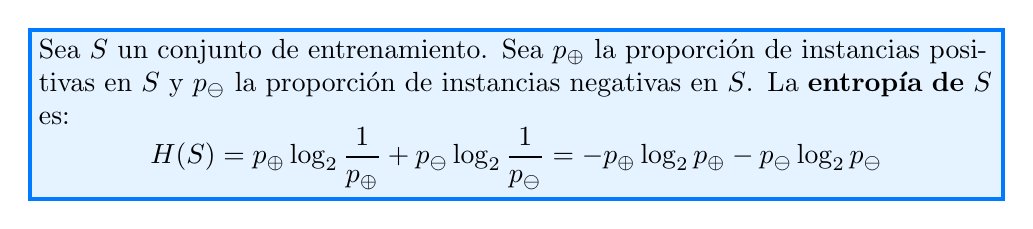
\begin{tikzpicture}
	\node[draw=lightblue, fill=lightblue!10, line width=1.5, text width=\linewidth] {Sea $S$ un conjunto de entrenamiento. Sea $p_\oplus$ la proporción de instancias positivas en $S$ y $p_\ominus$ la proporción de instancias negativas en $S$. La \textbf{entropía de $S$} es: \[ H(S)=p_\oplus\log_2\dfrac{1}{p_\oplus}+p_\ominus\log_2\dfrac{1}{p_\ominus}=-p_\oplus\log_2p_\oplus-p_\ominus\log_2p_\ominus \]};
\end{tikzpicture}

(Relación de la entropía con los conceptos de desorden, equiprobabilidad y homogeneidad).

La entropía nos mide la homogeneidad de los datos (relación inversa).
\begin{center}
	\includegraphics{"Temas/Tema 2/screenshot001"}
\end{center}
\begin{minipage}{0.45\textwidth}
	Para el caso binario:
	\begin{itemize}
		\item Entropía igual a 1 $\to$ mínima homogeneidad (equiprobabilidad: $p_\ominus=p_\oplus$).
		\item Entropía igual a 0 $\to$ máxima homogeneidad (todas las instancias de una clase)
	\end{itemize}
\end{minipage}\qquad\begin{minipage}{0.45\textwidth}
\begin{center}
	\includegraphics{"Temas/Tema 2/screenshot002"}
\end{center}
\end{minipage}
A la hora de construir un árbol es preferible crear nodos con nodos hoja homogéneos, es decir, de \textbf{baja entropía}.
\subsubsubsection{Ganancia de Información}
Sea un conjunto de datos $\mathcal{X}$ con entropía $H(\mathcal{X})$.

Si elegimos un atributo $A$ para crear un nodo del árbol, la entropía esperada es: \[ H(\mathcal{X},A)=\sum_{v\in\mathrm{valores}(A)}\dfrac{|\mathcal{X}_v|}{\mathcal{X}}H(\mathcal{X}_v) \]siendo $\mathcal{X}_v$ el subconjunto de $\mathcal{X}$ con todas las instancias con $A=v$.

Por lo tanto, la reducción esperada de la entropía, o lo que es lo mismo la \textbf{Ganancia de Información}, al elegir el atributo $A$ como nodo de decisión del árbol es \[ \bboxed{\mathrm{Ganacia}(\mathcal{X},A))H(\mathcal{X})-H(\mathcal{X},A)} \]
Por tanto, se elige el atributo que produzca hojas homogéneas, es decir, la \textbf{máxima} ganancia de información.

\Ej

Atributos nominales (no numéricos)

\begin{center}
	\begin{tabular}{|cccccc|}
		\hline
		\rowcolor[HTML]{A5FFC4} 
		\hline
		Día & Cielo & Temperatura & Humedad & Viento & \cellcolor[HTML]{FF8787}Jugar \\ \hline
		\rowcolor[HTML]{34CDF9} 
		\hline
		{\color[HTML]{333333} D1} & {\color[HTML]{333333} Soleado} & {\color[HTML]{333333} Calor} & {\color[HTML]{333333} Alta} & {\color[HTML]{333333} Flojo} & \cellcolor[HTML]{FF8787}No \\
		\rowcolor[HTML]{007AFF} 
		D2 & Soleado & Calor & Alta & Fuerte & \cellcolor[HTML]{FC5D5D}No \\
		\rowcolor[HTML]{34CDF9} 
		D3 & Nublado & Calor & Alta & Flojo & \cellcolor[HTML]{FF8787}Si \\
		\rowcolor[HTML]{007AFF} 
		D4 & Lluvia & Templado & Alta & Flojo & \cellcolor[HTML]{FC5D5D}Si \\
		\rowcolor[HTML]{34CDF9} 
		D5 & Lluvia & Frío & Normal & Flojo & \cellcolor[HTML]{FF8787}Si \\
		\rowcolor[HTML]{007AFF} 
		D6 & Lluvia & Ario & Normal & Fuerte & \cellcolor[HTML]{FC5D5D}No \\
		\rowcolor[HTML]{34CDF9} 
		D7 & Nublado & Ario & Normal & Fuerte & \cellcolor[HTML]{FF8787}Si \\
		\rowcolor[HTML]{007AFF} 
		D8 & Soleado & Templado & Alta & Flojo & \cellcolor[HTML]{FC5D5D}No \\
		\rowcolor[HTML]{34CDF9} 
		D9 & Soleado & Ario & Normal & Flojo & \cellcolor[HTML]{FF8787}Si \\
		\rowcolor[HTML]{007AFF} 
		D10 & Lluvia & Templado & Normal & Flojo & \cellcolor[HTML]{FC5D5D}Si \\
		\rowcolor[HTML]{34CDF9} 
		D11 & Soleado & Templado & Normal & Fuerte & \cellcolor[HTML]{FF8787}Si \\
		\rowcolor[HTML]{007AFF} 
		D12 & Nublado & Templado & Alta & Fuerte & \cellcolor[HTML]{FC5D5D}Si \\
		\rowcolor[HTML]{34CDF9} 
		D13 & Nublado & Calor & Normal & Flojo & \cellcolor[HTML]{FF8787}Si \\
		\rowcolor[HTML]{007AFF} 
		D14 & Lluvia & Templado & Alta & Fuerte & \cellcolor[HTML]{FC5D5D}No \\ \hline
	\end{tabular}
\end{center}
En el ejemplo del tenis tenemos 9 objetos clasificados como $\oplus$ y 5 como $\ominus$, con lo que \[ H([9\oplus,5\ominus])=-0.642\cdot\log_20.642-0.58\cdot\log_20.358=0.94 \]
\begin{center}
	\includegraphics{"Temas/Tema 2/screenshot003"}
\end{center}
Por lo tanto, el atributo que ofrece una mayor ganancia de información es el atributo \textbf{Cielo}.

Utilizando \textbf{Cielo} como nodo raíz el árbol inicial quedaría:
\begin{center}
	\includegraphics{"Temas/Tema 2/screenshot004"}
\end{center}
\begin{minipage}{0.45 \textwidth}
	Ahora habría que repetir el proceso con los nodos correspondientes a los valores \textbf{soleado} y \textbf{lluvia} (el nodo \textbf{nublado} sólo contiene una clase).
\end{minipage}\qquad\begin{minipage}{0.45\textwidth}
\begin{center}
	\includegraphics{"Temas/Tema 2/screenshot005"}
\end{center}
\end{minipage}

\begin{itemize}
	\item Para el nodo Cielo = Soleado:
	\begin{itemize}
		\item $\mathcal{X}_{\mathrm{soleado}}=\{D_1,D_2,D_8,D_9,D_11\}$ con $H(\mathcal{X}_{\mathrm{soelado}})=0.971$
		\item $\mathrm{Ganancia}(\mathcal{X}_{\mathrm{soleado}},\mathrm{Temperatura})=0.971-\dfrac{2}{5}\cdot0-\dfrac{2}{5}\cdot1-\dfrac{1}{5}\cdot0=0.570$
		\item $\mathrm{Ganancia}(\mathcal{X}_{\mathrm{soelado}},\mathrm{Humedad})=0.971-\dfrac{3}{5}\cdot0-\dfrac{2}{5}\cdot0=0.971$
		\item $\mathrm{Ganancia}(\mathcal{X}_{\mathrm{soleado}},\mathrm{Viento})=0.971-\dfrac{2}{5}\cdot1-\dfrac{3}{5}\cdot0.918=0.019$
	\end{itemize}
	\item Para el nodo Cielo = Lluvia:
	\begin{itemize}
		\item $\mathcal{X}_{\mathrm{lluvia}}=\{D_4,D_5,D_6,D_{10},D_{14}\}$ con $H(\mathcal{X}_{\mathrm{lluvia}})=0.971$
		\item $\mathrm{Ganancia}(\mathcal{X}_{\mathrm{lluvia}},\mathrm{Temperatura})=0.971-\dfrac{3}{5}\cdot0.918-\dfrac{2}{5}\cdot1-\dfrac{1}{5}\cdot0=0.820$
		\item $\mathrm{Ganancia}(\mathcal{X}_{\mathrm{lluvia}},\mathrm{Humedad})=0.971-\dfrac{2}{5}\cdot1-\dfrac{3}{5}\cdot0.918=0.820$
		\item $\mathrm{Ganancia}(\mathcal{X}_{\mathrm{lluvia}},\mathrm{Viento})=0.971-\dfrac{3}{5}\cdot0-\dfrac{2}{5}\cdot0=0.971$
	\end{itemize}
\end{itemize}

Por lo tanto, el árbol resultante sería
\begin{center}
	\includegraphics{"Temas/Tema 2/screenshot006"}
\end{center}
Todos los nodos hoja tienen una entropía nula (solo instancias de una clase).
\subsubsubsection{Error global}
Es la probabilidad de error, es decir, suma ponderada de los errores de todas las hojas del árbol. \[ E=\sum_{i=1}^{n_h}w_ie_i \]donde
\begin{itemize}
	\item $n_h$ es el numero de hojas del árbol.
	\item $w_i$ es el peso o probabilidad de la hoja $i$, es decir, la probabilidad de que una instancia sea clasificada por la partición representada por la rama que acaba en la hoja $i$.
	\item $e_i$ es el error correspondiente a la rama que acaba en la hoja $i$ (número de instancia erróneas que caen en la hoja $i$ entre el número de instancias que caen en la hoja $i$).
\end{itemize}
\subsubsubsection{Algoritmo}
El algoritmo básico de aprendizaje es el ID3 (Iterative Dichotomiser 3).

\begin{algorithm}
	\caption{árbol $\gets$ aprenderArbol(\textit{datos})}
	\begin{algorithmic}[1]
		\IF{todos los ejemplos en datos tienen la misma etiqueta}
		\RETURN un nodo hoja con dicha etiqueta
		\ELSE
		\STATE Sea $A$ el atributo que clasifica mejor a los objetos en datos
		\FORALL{posible valor $v$ de $A$}
		\STATE $data(v) \leftarrow$ todos los objetos con $A = v$
		\STATE Añadir nueva rama $\leftarrow$ aprenderArbol($data(v)$)
		\ENDFOR
		\RETURN árbol
		\ENDIF
	\end{algorithmic}
\end{algorithm}

\pagebreak

\textbf{ID3(Instancias, Etiquetas, Atributos)}

\begin{algorithmic}
	\REQUIRE \texttt{Instancias:} el conjunto de datos
	\REQUIRE \texttt{Etiquetas:} el conjunto de posibles clases.
	\REQUIRE \texttt{Atributos:} el conjunto de atributos en el conjunto \texttt{Instancias}.
	\IF{todas las instancias son positivas}
	\RETURN el nodo raíz con etiqueta $+$.
	\ELSIF{todas las instncias son negativas}
	\RETURN el nodo raíz con la etiqueta $-$.
	\ELSIF{\texttt{Atributos}=$\varnothing$}
	\RETURN el nodo raíz con el valor de \texttt{Etiquetas} más probable en \texttt{Instancias}.
	\ENDIF
	\STATE Sea $A$ el atributo que clasifica mejor las instancias en \textit{datos}.
	\STATE Crear un árbol con un nodo etiquetado con $A$
	\FORALL{posible valor $v_i$ del atributo $A$}
	\STATE añadir un arco bajo la raíz con la comprobación $A=v_i$.
	\STATE sea \texttt{Instancias} $v_i$ el subconjunto de \texttt{Instancias} con $A=v_i$.
	\IF{\texttt{Instancias}$_{v_i}=\varnothing$}
	\STATE añadir un nodo hoja al arco añadido con el valor de \texttt{Etiquetas} más probable en \texttt{Ejemplos}.
	\ELSE 
	\STATE añadir al nuevo árbol el subárbol generado por \textbf{ID3} (\texttt{Instancias}$_{v_i}$,\texttt{Etiquetas}, \texttt{Atributos}$-\{A\}$).
	\ENDIF
	\ENDFOR
	\RETURN nodo raíz
\end{algorithmic}
\subsubsection{Sobre-ajuste}
\subsubsubsection{Espacio de hipótesis y sobre-ajuste}
El \textbf{espacio de hipótesis} $H$ (no confundir con la entropía) en árboles de decisión
abarca todas las posibles combinaciones de atributos y valores que pueden formar
árboles de decisión, y nuestra tarea es encontrar la hipótesis más adecuada para
clasificar correctamente las instancias de entrada.

En general, se prefieren hipótesis cortas para evitar el sobre-ajuste (\textbf{overfitting}).

\begin{itemize}[label=\color{red}\textbullet, leftmargin=*]
	\item \color{lightblue}Sobre-ajuste
\end{itemize}
Dado un espacio de hipótesis $H$, se dice que una hipótesis particular $h\in H$ sobreajusta los datos de entrenamiento si existe un hipótesis alternativa $h'\in H$, tal que $h$ presenta un error menor que $h'$ sobre los ejemplos de entrenamiento, pero $h'$ presenta un error menor que $h$ sobre el conjunto total de observaciones.
\subsubsubsection{Proceso de poda}
\begin{itemize}[label=\color{red}\textbullet, leftmargin=*]
	\item \color{lightblue}¿Cómo podemos evitar el sobre-aprendizaje o sobre-ajuste?
\end{itemize}
\textbf{Poda:} Eliminar condiciones de las ramas del árbol encontrar más pequeños. Existe dos tipos de poda:\begin{itemize}
	\item \textbf{Prepoda:} El proceso se realiza durante la construcción del árbol, estableciendo un criterio de parada.
	\begin{itemize}
		\item El número de instancias por nodo.
		\item El error esperado.
		\item MDL (Minimun Description Lenght).
	\end{itemize}
	\item \textbf{Postpoda:} El proceso se realiza después de la construcción del árbol
	\begin{itemize}
		\item Consiste en ir eliminando nodos de abajo a arriba mientras se vaya cumpliendo un criterio determinado.
	\end{itemize}
\end{itemize}
Se pueden combinar ambas aproximaciones.
\subsubsubsection{Otras medidas}
\textbf{Medidas alternativas:} En algunos casos se suele utilizar otras medidas como:
\begin{itemize}
	\item El \textit{Ratio} de la ganancia de información, para evitar el hecho de que se favorece la selección de los atributos con más valores.
	\item MSE para regresión
	\item Índice Gini empleado por el algoritmo CART
	\item DKM, basados en AUC, MDL
\end{itemize}
\subsubsection{Algoritmo CART y Otros}
\subsubsubsection{CART}
\textbf{Cart} (\textbf{C}lasificación \textbf{A}nd \textbf{R}egression \textbf{T}rees). Similar al ID3 pero:
\begin{itemize}
	\item Permite que la variable que define la clase sea continua y no construye un conjunto de reglas.
	\item Utiliza el índice de Gini en vez de la ganancia de información para seleccionar el mejor atributo (la mejor partición).
	\item Utiliza también el esquema de partición recursiva utilizando una estrategia voraz.
	\item También permite resolver problemas de regresión.
\end{itemize}
Se elige la partición que produce el menor valor de la función de coste.
\begin{itemize}
	\item Para regresión: RSME.
	\item Para clasificación: GINI \[ \mathrm{Gini}(p)=\sum_{i=1}^{n}p_i(1-p_i) \] con $p_i$ las proposiciones de instancias de la clase $i$ en la partición.
\end{itemize}
Prepoda: Utiliza como criterio de parada el número mínimo de instancias asignadas al nodo.

Postpoda: Utiliza un criterio que controla la importancia relativa del error frente la complejidad (tamaño del árbol).
\subsubsubsection{C4.5, C5.0}
\textbf{C4.5:} Permite, a diferencia que ID3, que las características puedan ser continuas, definiendo de forma dinámica un atributo discreto particionando los atributos continuos en un conjunto discreto de intervalos.
\begin{itemize}
	\item C4.5 transforma los árboles obtenidos en un conjunto de reglas del tipo \textit{if-then}. La precisión de cada regla es evaluada de forma independiente para determinar el orden en el que deben ser aplicadas.
	\item Un proceso de poda elimina antecedentes de las reglas si con esto se mejora la precisión de la misma.
	\item C5.0, utiliza menos memoria y obtiene un conjunto de reglas menor y más preciso.
	\item J48 es la implementación en código abierto de C4.5
\end{itemize}
\subsubsection{Random Forests}
Random Forest es una técnica que construye un gran número de árboles de decisión no correlacionados.

Se basa en la técnica de Agregación de Bootstrap (Bagging), técnica de agregación de clasificadores o regresores que:
\begin{itemize}
	\item Aumenta la precisión y estabilidad reduciendo los efectos del ruido.
	\item Reduce la varianza en las predicciones.
	\item Ayuda a evitar el sobre ajuste.
\end{itemize}
La predicción del modelo se elige analizando las predicciones de cada uno de los árboles considerados en el modelo.
\subsubsubsection{Algoritmo}
\begin{algorithm}
	\caption{RF $\gets$ RandomForest(\textit{datos})}
	\begin{algorithmic}[1]
		\FOR{$i\gets1\to$ \textit{n_arboles}}
		\STATE Extraer una muestra de tamaño \textit{size(data)} de \textit{datos} por bootstrapping
		\STATE Construir un árbol $T_i$ repitiendo recursivamente para cada nodo hoja
		\STATE \begin{enumerate}[leftmargin=1.5cm]
			\item Seleccionar aleatoriamente $m$ atributos.
			\item Seleccionar la mejor partición de las inducidas por los $m$ atributos.
			\item Dividir el nodo en dos nodos hijos.
			\item Si el tamaño de nodo alcanza $n_{\min}$ no continuar dividiendo.
		\end{enumerate}
		\ENDFOR
		\RETURN El conjunto de árboles $\{T_i\}_1^{\text{\textit{n_arboles}}}$.
	\end{algorithmic}
\end{algorithm}

Si tenemos $p$ atributos las recomendaciones para el valor de $m$ son:
\begin{itemize}
\item Clasificación: $\lfloor\sqrt{m}\rfloor$

\item Regresión: $\lfloor p/3\rfloor$
\item Siendo el valor mínimo 1.
\end{itemize}
Una vez se han construido los árboles para hacer predicciones:
\begin{itemize}
	\item Clasificación: La clase más votada por los árboles.
	\item Regresión: La media de todas las predicciones
\end{itemize}
\subsubsubsection{OBB e importancia de las variables}
\textbf{OBB (out of the bag) error estime:} Para cada muestra se predice el error utilizando sólo los árboles en los que no ha sido utilizada (no ha sido elegida en bootstrapping)
\begin{itemize}
	\item Los valores son parecidos a los que se obtienen mediante una validación cruzada de $N$-pliegues.
\end{itemize}
\textbf{Importancia de los atributos:}
\begin{itemize}
	\item En cada partición del árbol se registra la mejora del criterio de división.
	\item Este valor se considera la importancia del atributo.
	\item Para cada variable se agregan los valores generados en cada árbol.
\end{itemize}
\subsubsection{Conclusiones}
La utilización de árboles de decisión es muy popular en muchas disciplinas.

Experimentalmente han demostrado una buena capacidad de clasificación.

La clave reside en la función a optimizar a la hora de elegir el atributo para disgregar el árbol.

Los ensambles nos permiten mejorar los resultados combinando información.
\subsubsection{Bosques Aleatorios (\textit{"Random Forest"})}
\subsubsubsection{Motivación}
Surgen para resolver el \textbf{"overfitting"} producido por los árboles de decisión.

El gran problema de los árboles de decisión: sesgo bajo y varianza alta.

Cambios imperceptibles en la distribución de los datos modifican totalmente la partición generada por un Árbol de Decisión (varianza alta).

\begin{center}
	\includegraphics{"Temas/Tema 2/screenshot007"}
	
	¿Cómo reducir la varianza?
\end{center}
\subsubsubsection{Solución}

\textbf{Muchos árboles} de decisión

\textbf{Aleatoriedad doble}
\begin{itemize}
	\item Conjuntos de entrenamiento 
\item Características 
\end{itemize}
\textbf{Agregación} de resultados 
\begin{itemize}
	\item Árboles malos, poco impacto en la predicción
\end{itemize}
\begin{center}
	\includegraphics{"Temas/Tema 2/screenshot008"}
	
	\includegraphics{"Temas/Tema 2/screenshot009"}
\end{center}
\subsubsubsection{Número de árboles}

\begin{minipage}{0.5\textwidth}
	Lo primero es fijar el \textbf{número de árboles}
	\begin{itemize}
		\item Normalmente es elevado, cientos.
	\item En este ejemplo, \textbf{5}
	\end{itemize}
	
	\hspace{2cm}
	
	Ruido en los datos afectará a algunos árboles
\end{minipage}\quad\begin{minipage}{0.5\textwidth}
\begin{center}
	\includegraphics[width=\linewidth]{"Temas/Tema 2/screenshot010"}
\end{center}
\end{minipage}
\subsubsubsection{Generación conjuntos de entrenamiento}
\begin{minipage}{0.5\textwidth}
\begin{center}
Una vez fijado el \textbf{número de árboles}, se construyen los conjuntos de entrenamiento.
	
	\begin{tikzpicture}
		\draw[double -latex=4pt colored by lightblue and lightblue] (0,0) -- (0,-1);
	\end{tikzpicture}
	
	{\Large \lb{\textbf{BOOSTRAPPING}}}
	
	Muestreo con reemplazo
\end{center}
\begin{itemize}[label=\color{red}\textbullet, leftmargin=*]
	\item \color{lightblue}Obtención de muestras \textbf{“Bootstrap”}
\end{itemize}

Supongamos un conjunto de datos $X$ (población) de tamaño $N$.
Se construyen muestras bootstrap de la población a partir de los datos:
\begin{enumerate}[label=\color{lightblue}\arabic*)]
	\item Elegir el tamaño de la muestra $N'\le N$.
	\item For $i=1:N'$
	\begin{enumerate}[label=\color{lightblue}\arabic*)]
		\item Elegir aleatoriamente una observación de $X$ con \textit{reemplazo}
		\item Añadirlo a la muestra
	\end{enumerate}
\end{enumerate}
En machine learning, $N'=N$.
\end{minipage}\qquad\begin{minipage}{0.45\textwidth}
\begin{center}
	\includegraphics[width=\linewidth]{"Temas/Tema 2/screenshot011"}
\end{center}
\end{minipage}
\begin{center}
	\includegraphics{"Temas/Tema 2/screenshot012"}
\end{center}

\subsubsubsection{Entrenamiento de los árboles}
Se introduce una \lb{segunda aleatoriedad} en la selección de las características que se emplean para realizar las particiones.
\begin{center}
	\includegraphics{"Temas/Tema 2/screenshot013"}
\end{center}

\begin{minipage}{0.5\textwidth}
	De la misma forma, se van entrenando (y construyendo) los demás árboles
\end{minipage}\quad\begin{minipage}{0.5\textwidth}
\begin{center}
	\includegraphics[width=\linewidth]{"Temas/Tema 2/screenshot014"}
\end{center}

\end{minipage}
\subsubsubsection{Modo operación}
\begin{center}
	\includegraphics{"Temas/Tema 2/screenshot015"}
\end{center}
\subsubsubsection{Bagging y Conjunto de Validación}

\textbf{Bagging:} es la la combinación del bootstrapping y la agregación, que es precisamente el nombre genérico con que se conoce a los algoritmos como los Bosques Aleatorios y otros similares.

\lb{\textbf{Conjunto de validación o "out-of-bag":}} se emplea para selección de hiperparámetros
\begin{center}
	\begin{tabular}{rl}
		$\dfrac{1}{N}$ & $\to$ probabilidad de seleccionar una instancia\\
		$1-\dfrac{1}{N}$ & $\to$ probabilidad de que no se seleccione una instancia\\
		$\left(1-\dfrac{1}{N}\right)^N\approx e^{-1}=0.368$ & $\to$ probabilidad que una instancia no se seleccione tras $N$ veces
	\end{tabular}
	
	\begin{tabular}{ll}
		Por tanto, aproximadamente: & conjunto de \textbf{validación} ("out-of-bag") $\to 36.8\%$\\
		&conjunto de \textbf{entrenamiento} $\to63.2\%$
	\end{tabular}
\end{center}
\subsubsubsection{Selección del número de árboles}
\begin{minipage}{0.4\textwidth}
Se fija el número de características y el criterio de parada, y se entrenan múltiples bosques cambiando progresivamente el número de árboles que lo conforman.

Se selecciona el que menor error de validación proporciona.

Usualmente, en aplicaciones prácticas, se usan entre 100 y 200 árboles
\end{minipage}\qquad\begin{minipage}{0.55\textwidth}
\begin{center}
	\includegraphics[width=\linewidth]{"Temas/Tema 2/screenshot016"}
\end{center}

\end{minipage}
\subsubsubsection{Seleccionar del número de características}
\begin{minipage}{0.4\textwidth}
	Con el número de árboles ya
	determinado, fijamos el
	criterio de parada y repetimos
	el procedimiento cambiando
	el número de características, y
	escogemos aquel que genere
	el menor error.
\end{minipage}\qquad\begin{minipage}{0.55\textwidth}
\begin{center}
	\includegraphics[width=\linewidth]{"Temas/Tema 2/screenshot017"}
\end{center}

\end{minipage}
\subsubsubsection{Selección del criterio de parada}
\begin{minipage}{0.4\textwidth}
Finalmente, con el número de árboles
y de características fijo, variamos el
criterio de parada y escogemos el que
arroje el menor error. El criterio de
parada puede ser, por ejemplo, el
mínimo número de datos de una hoja
(algún método de prepoda).
\end{minipage}\qquad\begin{minipage}{0.55\textwidth}
\begin{center}
	\includegraphics[width=\linewidth]{"Temas/Tema 2/screenshot018"}
\end{center}

\end{minipage}
\subsubsubsection{Relevancia de las características}
\begin{minipage}{0.5\textwidth}
	Los valores de los índice Gini (para el caso de la clasificación)
o el error cuadrático medio (para el caso de la regresión)
aportan una medida de la bondad de la partición hecha en
cada nodo. Con estos valores, se puede establecer un \textbf{orden de importancia} de las características. 
\end{minipage}\qquad\begin{minipage}{0.5\textwidth}
\begin{center}
	\includegraphics[width=\linewidth]{"Temas/Tema 2/screenshot019"}
\end{center}
\end{minipage}
\begin{center}
	\includegraphics{"Temas/Tema 2/screenshot020"}
\end{center}
\subsection{Perceptrón monocapa y multicapa (MLP)}
\subsubsection{Teoría de la decisión}
Tres escenarios para resolver un problema de decisión
\begin{itemize}
	\item \textbf{Decisión analítica.} Se fundamentan en la teoría bayesiana para inferir las probabilidades a posteriori de las las clases
	\item \textbf{Modelos discriminatorios.} Infieren directamente las probabilidades a posteriori.
	\item \textbf{Funciones discriminantes.} Encuentran una función $f(x)$ que mapea directamente una entrada $x$ a una determinada clase.
\end{itemize}
\subsubsubsection{Decisión analítica}
Se fundamentan en la inferencia de $p(\mathrm{x}|C_k)$ y $p(C_k)$ (o, equivalente $p(\mathbf{x},C_k)$).

\begin{minipage}{0.5\textwidth}
	Procedimiento:
	\begin{enumerate}[label=\color{lightblue}\arabic*)]
		\item A partir de los datos, se infieren verosimilitudes y probabilidades a priori: $p(\mathbf{x}|C_k)$ y $p(C_k)$.
		\item Se aplica el Teorema de Bayes para calcular las probabilidades a posteriori \[ p(C_k|\mathrm{x})=\dfrac{p(\mathrm{x}|C_k)p(C_k)}{p(\mathrm{x})}=\dfrac{p(\mathrm{x}|C_k)p(C_k)}{\displaystyle\sum_kp(\mathrm{x}|C_k)p(C_k)} \]
		\item Se emplea la teoría de la decisión para determinar la clase de una entrada $x$
	\end{enumerate}
	Los métodos que explícita o implícitamente modelan las distribuciones de las entradas así como las salidas, $p(\mathrm{x},C_k)$, se llaman \textbf{modelos generativos} pues mediante \textit{muestreo} se pueden generar datos sintéticos.
\end{minipage}\qquad\begin{minipage}{0.5\textwidth}
\begin{center}
	\includegraphics{"Temas/Tema 2/screenshot021"}
\end{center}
\end{minipage}
\subsubsubsection{Modelos discriminatorios}
Producen directamente una estima de las probabilidades a posteriori de las clases para una entrada dada.
\begin{enumerate}[label=\color{lightblue}\arabic*)]
	\item El procedimiento ahora consiste en, con los datos disponibles, diseñar y entrenar un modelo que minimice una determinada función de error entre las entradas y sus salidas deseadas
	\item Las salidas del modelos representan, mediante algún código, las probabilidades a posteriori de las clases para la entrada dada.
	\item El ejemplo más claro de modelos discriminativos son las \textbf{redes neuronales progresivas} como, por ejemplo, los MLPs entrenados para minimizar la entropía cruzada con unidades de salida tipo softmax
\end{enumerate}
\begin{center}
	\includegraphics{"Temas/Tema 2/screenshot022"}
\end{center}
\subsubsubsection{Funciones discriminantes}
Encuentran una función $f(x)$, llamada \textit{función discriminante}, que directamente mapea cada entrada $x$ a la etiqueta de una clase.

\begin{minipage}{0.5\textwidth}
	\begin{itemize}[label=\color{red}\textbullet, leftmargin=*]
		\item \color{lightblue}Ejemplo: problema de dos clases
	\end{itemize}
	\[ \begin{array}{ll}
		f(x)=1, & \text{si }y(x)=\mathrm{w}^\intercal\mathrm{x}+w_0>0\\
		f(x)=0, & \text{si }y(x)=\mathrm{w}^\intercal\mathrm{x}+w_0<0
	\end{array} \]
\end{minipage}\qquad\begin{minipage}{0.5\textwidth}
\begin{center}
	\includegraphics[width=\linewidth]{"Temas/Tema 2/screenshot023"}
\end{center}

\end{minipage}
\subsubsection{Fundamento biológico}
Membrana permeable para ciertas sustancias iónicas. Se crea una diferencia de potencial.

\begin{center}
	\includegraphics{"Temas/Tema 2/screenshot024"}
\end{center}
Tras la activación sináptica, se propagan diferencias de potencial.entre el soma y el entorno.
\begin{center}
	\includegraphics{"Temas/Tema 2/screenshot025"}
\end{center}
\subsubsection{Perceptrón monocapa}
\subsubsubsection{(Widrow): filtro transversal (adaptativo) + umbral duro}
\begin{center}
	\includegraphics{"Temas/Tema 2/screenshot026"}
\end{center}
\begin{minipage}{0.5\textwidth}
	División según hiperplano: \[ z=\mathbf{w^\intercal x}+b=0 \]donde la \lb{Función discriminante} (lineal) es \[ z=\mathbf{w^\intercal x}+b \]
\end{minipage}\qquad\begin{minipage}{0.5\textwidth}
\begin{center}
	\includegraphics{"Temas/Tema 2/screenshot027"}
\end{center}
\end{minipage}
\subsubsubsection{(Rosenblatt): dados $N$ pares entrada-salida: $\{\mathbf{x}_k,\mathbf{d}_k\}_1^N$}
Muestra a muestra: \[ \mathbf{w}(k+1)=\mathrm{w}(k)+\dfrac{\alpha}{2}(d_k-o_k)x_k,\quad(\alpha>0) \]
Bloque: \[ \mathrm{w}(m+1)=\mathrm{w}(m)=\dfrac{\alpha}{2}\sum_{k=1}^{N}(d_k-o_k(m))\mathrm{x}_k,\quad(\alpha>0) \]
Es aprendizaje:
\begin{itemize}
	\item \textbf{Supervisado:} pares de entrenamiento dados.
	\item \textbf{No lineal:} se emplea la salida $(o)$ en el error.
	\item \textbf{Hebbiano:} refuerza las intervenciones correctas ($\pm\alpha\mathrm{x}_k$ en $\mathbf{w}$ según el signo del error).
\end{itemize}
Solo converge si hay separabilidad lineal

Ejemplo gráficos: $D=2,b=0$ y una muestra $\{\mathbf{x}_k,\lbb{d_k=-1}{\text{salida deseada}}\}$
\begin{center}
	\includegraphics[width=\linewidth]{"Temas/Tema 2/screenshot028.drawio"}
\end{center}

Las rectas narajas y amarillan se sacan sumando a $\mathrm{w}(k+1)$ y $\mathrm{w}(\alpha)$ respectivamente el $-\alpha x$.

Es decir, aplicando la fórmula de muestra a muestra.
\subsubsection{Limitaciones del Perceptron Monocapa}
Minskey y Papert: es un "solo" \textbf{discriminante lineal}, capaz de resolver problemas de juguete (por ejemplo OREX).
\begin{center}
	\includegraphics{"Temas/Tema 2/screenshot029"}
\end{center}
Si se dispone en capas: gradiente imposible por el umbral duro.

La ya comentada falta de convergencia.
\subsubsection{El algoritmo LMS}
(Widrow y Hopf): proponen emplear $z$ en el error en lugar de $o$ y minimizar el coste cuadrático (Least Mean Square) por gradiente: \[ \min_{\mathrm{x}}C(\mathrm{w})=\min_{\mathrm{w}}\dfrac{1}{2}\sum_{k=1}^{N}(d_k-z_k)^2 \]
\begin{itemize}
	\item Muestra a muestra: \[ \mathrm{w}(k+1)=\mathrm{w}(k)+\alpha(d_k-z_k)\mathrm{x}_k,\quad(\alpha>0) \] (más rápido, pero más ruidoso).
	\item Bloque: \[ \mathrm{w}(m+1)=\mathrm{w}(m)+\alpha\sum_{k=1}^{N}(d_k-z_k(m))\mathrm{x}_k,\quad(\alpha>0) \]
\end{itemize}

Para entradas independientes de valores independientes de media cero y autocorrelación $R_{\mathrm{xx}}$, converge a la solución MMSE (solución de Wiener-Hopf) \[ \mathrm{x}_{opt}=R_{xx}^{-1}\mathtt{E}\{\dx\}\text{ si }\alpha<\dfrac{2}{\lambda_{\max}} \]
\subsubsection{Características del LMS}
El LMS es muy robusto: converge en muchos casos

Aprendizaje:
\begin{itemize}
	\item \textbf{Supervisado}
	\item \textbf{Lineal:} se emplea la salida $(\mathbf{z})$ en el error
	\item Por prestaciones: según coste cuadrático
\end{itemize}
Produce resultados razonables (los mejores mediante una frontera lineal) aunque el problema no se separable linealmente.

\textbf{NLMS ó Delta-LMS:} $\alpha\longrightarrow\dfrac{\alpha}{\|\mathbf{x}\|^2}$, independiza de la energía de las muestras.
\subsubsection{Error cuadrático (SSE) para clasificación}
\subsubsubsection{Problema con los "OUTLIERS"}
\begin{center}
	\includegraphics{"Temas/Tema 2/screenshot030"}
\end{center}
La figura muestra el resultado obtenido por el LMS (en morado) para dos situaciones distintas.
\subsubsection{Activación blanda}
El \textbf{umbral duro} de Widrow, se cambia por una \textbf{aproximación derivable}

Resulta adecuada la forma sigmoidal o sigmoide:

\begin{minipage}{0.5\textwidth}
	\begin{itemize}
		\item \textbf{Función logística:} \[ o=f(z)=\dfrac{1}{1+e^{-gz}} \]
		\item \textbf{Tangente hiperbólica} ($\tanh$): \[ o=f(z)=\dfrac{1-e^{-gz}}{1+e^{-gz}}=\tanh\left(\dfrac{gz}{2}\right) \]
	\end{itemize}
\end{minipage}\qquad\begin{minipage}{0.5\textwidth}
\begin{center}
	\includegraphics[scale=0.8]{"Temas/Tema 2/screenshot031"}
\end{center}
\end{minipage}

$g$: saturación (determina la pendiente de la sigmoide en $z=0$).

En principio, asumible por los pesos.
\subsubsection{LMS con activación blanda}
Ahora: $z\to o$: \[ \min_{\mathrm{w}}C(\mathrm{w})=\min_{\mathrm{w}}\dfrac{1}{2}\sum_{k=1}^{N}(d_k-o_k)^2 \]
\begin{itemize}
	\item Muestra a muestra: \[ \mathrm{w}(k+1)=\mathrm{w}(k)+\alpha(d_k-o_k)f'(z_k)\mathrm{x}_k,\quad(\alpha>0) \]
	\item Bloque: \[ \mathrm{w}(m+1)=\mathrm{w}(m)+\alpha\sum_{k=1}^{N}(d_k-o_k(m))f'(z_k(m))\mathrm{x}_k,\quad(\alpha>0) \]
\end{itemize}
Aparece un factor $f'(z_k)$ que se puede calcular a partir de la propia salida según:

\begin{minipage}{0.5\textwidth}
	\begin{itemize}
		\item Para función logística: $f'(z)=go(1-o)$
	
	\[ \begin{aligned}
		\text{Demo: }f'(z)&=\dfrac{ge^{-gz}}{(1+e^{-gz})^2}=g\dfrac{1}{(1+e^{-gz})}\dfrac{e^{-gz}}{(1+e^{-gz})}\\
		&=g\dfrac{1}{(1+e^{-gz})}\left(1-\dfrac{1}{(1+e^{-gz})}\right)\\
		&=go(1-o)
	\end{aligned} \]
	\item Para $\tanh:\:f'(z)=\dfrac{1}{2}g(1-o^2)$
	\end{itemize}
\end{minipage}\qquad\begin{minipage}{0.5\textwidth}
\begin{center}
	\includegraphics{"Temas/Tema 2/screenshot031"}
\end{center}
\end{minipage}
\subsubsection{Arquitectura del Perceptron Multicapa (MLP)}
\subsubsubsection{Redes Multicapa}
\begin{center}
	\includegraphics{"Temas/Tema 2/screenshot032"}
\end{center}
\subsubsection{Propiedades de las MLP}
Son:
\begin{itemize}
	\item potentes
	\item versátiles
	\item distribuidas: robustas
	\item paralelas: rápidas (entrenadas)
\end{itemize}
pero:
\begin{itemize}
	\item de entrenamiento difícil y lento
	\item de difícil análisis
\end{itemize}
\subsubsection{Capacidades del MLP}
\begin{center}
	\includegraphics[width=\linewidth]{"Temas/Tema 2/screenshot033"}
\end{center}
Para MLPs con dos capas ($L = 2$), se han probado los siguientes teoremas:

Cybenko: basta con una capa oculta de unidades sigmoidales (en número indefinido) para \begin{center}
	$R^{N_0}\longrightarrow(1,-1)^{N_L}$\quad(Clasificación)
\end{center} donde $N_0$ y $N_L$ son la dimensión de la entrada y la salida, respectivamente.

Kolmogorov (adaptado por Hetch-Nielsen): basta con una capa oculta de $2N_0 + 1$ unidades de activaciones adecuadas para \begin{center}
	$(1,-1)^{N_0}\longrightarrow R^{N_L}\quad$(Regresión)
\end{center}
\subsubsection{Notación utilizada MLP}
\begin{center}
	\includegraphics{"Temas/Tema 2/screenshot034"}
\end{center}
\subsubsection{Algoritmo de retropropagación (BackPropagation (BP))}
Básicamente consiste en dos fases:
\begin{itemize}
	\item \textbf{Hacia adelante:} primero se aplica una instancia a las entradas de la red y su efecto se propaga a través de la misma, capa a capa, hasta la salida.
	\item \textbf{Hacia atrás (BP):} Después, se re-calculan los pesos mediante el gradiente del error. En concreto, se calcula el valor de la función de error, que compara la respuesta actual de la red y la respuesta deseada, y este error se propaga hacia atrás.
\end{itemize}
El objetivo es minimizar \[ \min_{\mathrm{w}}C(\mathrm{w})=\min_{\mathrm{w}}\dfrac{1}{2}\sum_{m=1}^{N}(\mathbf{d}_m-\mathbf{o}_m)^2 \] donde $\mathbf{w}$ representa todos los pesos de la red y $m$ la muestra o instancia.

Algoritmo de gradiente \[ w_{ji}^{(l)}(k+1)=e_{ji}^{(l)}(k)-\eta\dfrac{\partial C}{\partial w_{ji}^{(l)}}(k) \]
Para cada iteración $k$, se tienen las ecuaciones siguientes $\dfrac{\partial C}{\partial w_{ji}^{(l)}}=\dfrac{\partial C}{\partial o_j^{(l)}}\dfrac{\partial o_j^{(l)}}{\partial w_{ji}^{(l)}}=\dfrac{\partial C}{\partial o_j^{(l)}}f_j^{\prime(l)}o_i^{(l-1)}=\Delta_j^{(l)}o_i^{(l-1)}$ ya que \linebreak $o_j^{(l)}=f\left(\sum_{k=1}^{N_{l-1}}e_{jk}^{(l)}o_k^{(l-1)}\right)$
\begin{equation}
	\begin{split}
	\Delta_j^{(l)}&=\left(\sum_{n_{l+1}}^{N_{l+1}}\dfrac{\partial C}{\partial o_{n_{l+1}}^{(l+1)}}\dfrac{o_{n_{l+1}}^{(l+1)}}{\partial o_j^{(l)}}\right)f_j^{\prime(l)}=\left(\sum_{n_{l+1}}^{N_{l+1}}\dfrac{\partial C}{\partial o_{n_{l+1}}^{(l+1)}}f_{n_{l+1}}^{\prime(l+1)}w_{n_{l+1}j}^{(l+1)}\right)f_j^{\prime(l)}\\
	&=\left(\sum_{n_{l+1}}^{N_{l+1}}\Delta_{n_{l+1}}^{(l+1)}w_{n_{l+1}j}^{(l+1)}\right)f_j^{\prime(l)}
\end{split}
\end{equation}
BackPropagation (también Regla Delta Generalizada)) \[ w_{ji}^{(l)}(k+1)=w_{ji}^{(l)}-\eta\Delta_j^{(l)}(k)o_i^{(l-1)}(k) \]
Se procede: \[ l=L\longrightarrow L-1,L-2,\dots,1\quad\text{(¡retroprogramación!)} \] insertando gradiente y considerando que
\begin{itemize}
	\item Para $l=L$ se aplica \[ \Delta_j^L=\dfrac{\partial C}{\partial o_j^{(L)}}f_j^{\prime (L)} \]
	\item Y para $l<L$, se aplica (1)
\end{itemize}
Recuérdese que, para sigmoides, las derivadas dependen solo de los salidas: $f'(z)=go(1-o)$ para función logística y $f'(z)=\dfrac{1}{2}g(1-o^2)$ para $\tanh$.
\subsubsection{Modos de entrenamiento}
\begin{itemize}[label=\color{red}\textbullet, leftmargin=*]
	\item \color{lightblue}¿Cada cuanto se actualizan los pesos?
\end{itemize}
\begin{itemize}
	\item \lb{Batch:} depués de cada época del conjunto de entrenamiento.
	\item \lb{Mini-Batch:} despuñes de una muestra (conjunto de patrones) del conjunto de entrenamiento.
	\item \lb{Online:} depués de cada ejemplo.
\end{itemize}
\begin{center}
	\includegraphics{"Temas/Tema 1/Screenshot030"}
\end{center}
\subsubsection{Sobre las muestras}
Conjunto de muestras de entrenamiento \lb{representativo}

Conviene \lb{preprocesar} las muestras para eliminar información que de seguro se sabe irrelevante

Conviene \lb{normalizar} (características con media nula y varianza unidad)

Pueden ser útiles \lb{códigos sencillos} (en general, las NNs muestran sensibilidad al formato de presentación). Ejemplos: 1:N, termómetro, etc.

Para el mini-batch y online, conviene \lb{Aleatorizar} el orden de presentación de las muestras y \lb{ciclar} las series de entrenamiento.

\newpage

\section{El concepto de integral de Riemann y sus propiedades}
\subsection{Función integrable}
\begin{itemize}[label=\color{red}\textbullet, leftmargin=*]
	\item \color{lightblue}Definición
\end{itemize}
Dado $[a,~b]$ un intervalo de la recta real, se define una partición $\mathcal{P}$ de dicho intervalo como una sucesión finita de números reales de la forma \[ a=x_0<x_1<x_2<\cdots<x_{n-1}<x_n=b. \]A cada uno de los intervalos de la forma $[x_i,~x_{i+1}]$ con $i=0,1,\hdots,n-1$ se les conoce como intervalos de la partición $\mathcal{P}$. Se define el diámetro de la partición $\mathcal{P}$ como \[ \mathrm{diam}(\mathcal{P})=\max\{|x_{i+1}-x|:i=0,1,\hdots,n-1\}. \]Dadas dos particiones $\mathcal{P}$ y $\mathcal{P}'$ de un intervalo $[a,~b],~\mathcal{P}$ se dice más fina que $\mathcal{P}'$ si todo elemento de $\mathcal{P}$. Se verifica entonces que $\mathrm{diam}(\mathcal{P})\le\mathrm{diam}(\mathcal{P}')$.
\begin{itemize}[label=\color{red}\textbullet, leftmargin=*]
	\item \color{lightblue}Definición
\end{itemize}
Sea $f:[a,~b]\rightarrow\mathbb{R}$ una función real de variable real. Se define la suma inferior de Riemann de $f$ para la partición $\mathcal{P}$ como \[ s(\mathcal{P},f,[a,~b]) =\sum_{i=0}^{n-1}m_i\cdot(x_{i+1}-x_i),\] donde $m_i=\mathrm{inf}\{f(x):x\in[x_i,~x_{i+1}]\}$. Geométricamente, la suma inferir de Riemann coincide con la suma de las áreas de los rectángulos.

Se define la suma de Riemann de $f$ en la partición $\mathcal{P}$ como \[ S(\mathcal{P},f,[a,~b]) =\sum_{i=0}^{n-1}M_i\cdot(x_{i+1}-x_i),\] donde $M_i=\sup\{f(x):x\in[x_i,~x_{i+1}]\}$.

Es claro que \[ s(\mathcal{P},f,[a,~b]) =\le S(\mathcal{P},f,[a,~b]).\] Además si $\mathcal{P}'$ es más fina que $\mathcal{P}$ tenemos: \[ \begin{array}{l}
	s(\mathcal{P},f,[a,~b])\le s(\mathcal{P}',f,[a,~b])\\
	S(\mathcal{P},f,[a,~b])\le S(\mathcal{P}',f,[a,~b])
\end{array} \]
\begin{itemize}[label=\color{red}\textbullet, leftmargin=*]
	\item \color{lightblue}Definición
\end{itemize}
 Sea $(\mathcal{P}_n)_n$ una sucesión de particiones de manera que $\mathcal{P}_{n+1}$ es más fina que $\mathcal{P}_n$ para cada $n\in\mathbb{N}$ y de manera que $\lim_{n\to\infty}\mathrm{diam}(\mathcal{P}_n)=0$. Diremos que una función es integrable Riemann en $[a,~b]$ o integrable en $[a,~b]$ si existen y son iguales los límites \[ \lim_{n\to\infty}s(\mathcal{P}_n,f,[a,~b]) =\lim_{n\to\infty}S(\mathcal{P}_n,f,[a,~b])\] Dicho límite se denotará como \[ \int_{a}^{b}f(x)\mathrm{d}x=\lim_{n\to\infty}s(\mathcal{P}_n,f,[a,~b])=\lim_{n\to\infty}S(\mathcal{P}_n,f,[a,~b]) ,\] y se denomina integral de Riemann de $f$ en $[a,~b]$.

Geométricamente se observa que cuando la función es positiva, dicho límite coincide con el área de la superficie definida por la gráfica, el eje $OX$ y las rectas $x=a$ y $x=b$. ¿Cuándo $f$ es integrable? Estos son algunos resultados:
\begin{itemize}[label=\color{red}\textbullet, leftmargin=*]
	\item \color{lightblue}Teorema
\end{itemize}
Sea $f:[a,~b]\rightarrow\mathbb{R}$ una función, entonces $f$ es integrable en $[a,~b]$.

Sea $f:[a,~b]\rightarrow\mathbb{R}$ una función acotada con un número finito de puntos de discontinuidad, entonces $f$ es integrable en $[a,~b]$.
\subsection{Propiedades de la Integral de Riemann}
\begin{itemize}[label=\color{red}\textbullet, leftmargin=*]
	\item \color{lightblue}Proposición
\end{itemize}
Sea $f:[a,~b]\rightarrow\mathbb{R}$ integrable. Entonces se verifican las siguientes propiedades: 
\begin{enumerate}[label=\arabic*)]
	\item $\int_{a}^{a}f(x)\mathrm{d}x=0$.
	\item Si $c\in(a,~b)$ entonces $\int_a^bf(x)\mathrm{d}x=\int_a^cf(x)\mathrm{d}x+\int_c^bf(x)\mathrm{d}x$.
	\item $\int_a^bf(x)\mathrm{d}x=-\int_b^af(x)\mathrm{d}x$.
\end{enumerate}
\begin{itemize}[label=\color{red}\textbullet, leftmargin=*]
	\item \color{lightblue}Propiedades
\end{itemize}
Sea $f,g:[a,~b]\rightarrow\mathbb{R}$ dos funciones integrables. Entonces se verifican las siguientes propiedades:
\begin{itemize}
	\item $f+g$ es integrable en $[a,~b]$, \[ \int_a^b(f(x)+g(x))\mathrm{d}x=\int_a^bf(x)\mathrm{d}x+\int_a^bg(x)\mathrm{d}x. \]
	\item Para cada $\alpha\in\mathbb{R},~\alpha\cdot f$ es integrable en $[a,~b]$, \[ \int_{a}^{b}\alpha\cdot f(x)\mathrm{d}x=\alpha\cdot\int_{a}^{b}f(x)\mathrm{d}x. \]
	\item Si $f(x)\ge0$ para cada $x\in[a,~b]$, entonces \[ \int_a^bf(x)\mathrm{d}x\ge0. \]
	\item Si $f(x)\ge g(x)$ para cada $x\in[a,~b]$ entonces \[ \int_a^bf(x)\mathrm{d}x\ge\int_a^bg(x)\mathrm{d}x. \]
	\item La función $|f|$ es integrable en $[a,~b]$ y \[ \left|\int_a^bf(x)\mathrm{d}x\right| \le\int_a^b|f(x)|\mathrm{d}x.\]
\end{itemize}
\subsection{Teorema de la Media Integral}
\begin{itemize}[label=\color{red}\textbullet, leftmargin=*]
	\item \color{lightblue}Proposición
\end{itemize}
Sea $F$ una función integrable en $[a,~b]$ y sean $m$ y $M$ los valores mínimos y máximos respectivamente de la función $f$ en ese intervalo, entonces se verifica que \[ m(b-a)\le\int_{a}^{b}f(x)\mathrm{d}x\le M(b-a). \]
\begin{itemize}[label=\color{red}\textbullet, leftmargin=*]
	\item \color{lightblue}Teorema
\end{itemize}
Si $f$ es una función continua en un intervalo $[a,~b]$, entonces existe un punto $c\in[a,~b]$ tal que \[ \int_a^bf(x)\mathrm{d}x=(b-a)f(c). \] Al valor $f(c)$ se le denomina valor medio de $f$ en $[a,~b]$.
\subsection{El teorema Fundamental del Cálculo Integral}
Sea $f:[a,~b]\rightarrow\mathbb{R}$ una función integrable en $[a,~b]$ y continua en $x_0\in(a,~b)$, entonces la función $F$ definida en (1) es derivable en $x_0$ y se verifica que \[ F'(x_0)=f(x_0). \]
En general, si la función $f$ es continua en $[a,~b]$ entonces $F$ es derivable en $(a,~b)$ y $F'(x)=f(x)$ para cada $x\in(a,~b)$.
\subsection{Regla de Barrow}
Dadas $f,G:[a,~b]\rightarrow\mathbb{R}$, diremos que $G$ es una función \textit{primitiva} de $f$ si se verifica que $G'(x)=f(x)$ para cada $x\in[a,~b]$.

El Teorema Fundamental del Cálculo Integral afirma que si $f$ es continua en $[a,~b]$ entonces existe una función primitiva.

Las primitivas son únicas salvo constantes, es decir, si $G-1,G_2:[1,~b]\rightarrow\mathbb{R}$ son primitivas de $f$ entonces $G_1(x)=G_2(x)+k$ para cada $x\in[a,~b]$, donde $k$ es una constante real.
\begin{itemize}[label=\color{red}\textbullet, leftmargin=*]
	\item \color{lightblue}Proposición
\end{itemize}
Sea $G:[a,~b]\rightarrow\mathbb{R}$ una primitiva de una función $f:[a,~b]\rightarrow\mathbb{R}$ entonces \[ \int_a^bf(x)\mathrm{d}x=G(d)-G(a). \]
\subsection{Integrales impropias}
\subsubsection{Integrales impropias de primera especia}
\begin{itemize}[label=\color{red}\textbullet, leftmargin=*]
	\item \color{lightblue}Definición 
\end{itemize}
Sea $f:[a,~+\infty]\rightarrow\mathbb{R}$ una función integrable en cada intervalo $[a,~b]$ con $b\in[a,~+\infty)$. Se define la integral impropia \[ \int_a^\infty f(x)\mathrm{d}x =\lim_{b\to\infty}\int_a^bf(x)\mathrm{d}x.\]
Si el límite anterior existe y es finito la integral se dice que es convergente, si el límite existe pero es $\pm\infty$ la integral es divergente. Si el límite no existe diremos que la integral es oscilante.

De forma análoga se define la integral impropia \[ \int_{-\infty}^bf(x)\mathrm{d}x=\lim_{a\to-\infty}\int_a^bf(x)\mathrm{d}x. \]
La integral \[ \int_{-\infty}^{+\infty}f(x)\mathrm{d}x.=\int_{-\infty}^{a}f(x)\mathrm{d}x+\int_{a}^{+\infty}f(x)\mathrm{d}x. \]
El valor de $\int_{-\infty}^{+\infty}f(x)\mathrm{d}x$ no depende del punto $a\in\mathbb{R}$.

Se define valor principal de la integral impropia de $f$ en $(-\infty,+\infty)$ como el límite \[ \mathrm{V.P.}\int_{-\infty}^{+\infty}f(x)\mathrm{d}x=\int_{-t}^{t}f(x)\mathrm{d}x. \]
Si la integral es convergente, el valor principal de la integral y la integral coinciden, mientras que en el caso en el que no sea convergente esto no tiene por qué suceder.
\begin{itemize}[label=\color{red}\textbullet, leftmargin=*]
	\item \color{lightblue}Ejemplo
\end{itemize}
Consideramos la función $f(x)=x$. Puesto que $\int_{-t}^{t}x\mathrm{d}x=0$, así \[ \mathrm{V.P.} \int_{-\infty}^{+\infty}x\mathrm{d}x=\lim_{t\to-\infty}x\mathrm{d}x=0,\] mientras que \[ \int_{-\infty}^{+\infty}x\mathrm{d}x\text{ no existe.} \]
\subsubsection{Criterios de convergencia I}
\textcolor{lightblue}{\underline{Criterio de comparación}}

\begin{itemize}[label=\color{red}\textbullet, leftmargin=*]
	\item \color{lightblue}Proposición (Criterios de comparación)
\end{itemize}
Sea $f,g:[a,~\infty)\rightarrow\mathbb{R}$ dos funciones positivas e integrales en $[a,~b]$, para todo $b\in[a,~\infty)$. Si $f(x)\ge g(x)$ para cada $x\in[a,~\infty)$ se satisfacen las siguientes propiedades:

\begin{enumerate}[label=\arabic*)]
	\item Si $\int_{a}^{+\infty}f(x)\mathrm{d}x$ es convergente, entonces $\int_{a}^{+\infty}g(x)\mathrm{d}x$ es convergente.
	\item Si $\int_{a}^{+\infty}g(x)\mathrm{d}x$ es divergente, entonces $\int_{a}^{+\infty}f(x)\mathrm{d}x$ es divergente.
\end{enumerate}
\begin{itemize}[label=\color{red}\textbullet, leftmargin=*]
	\item \color{lightblue}Proposición (Criterio del límite)
\end{itemize}
Sea $f,g:\left[a,~\infty\right)\rightarrow\mathbb{R}$ dos funciones positivas e integrales en $[a,~b]$, para todo $b\in[a,~\infty)$. Sea $\infty\neq I=\lim_{x\to\infty}\dfrac{f(x)}{g(x)}$. Entonces: 
\begin{enumerate}[label=\arabic*)]
	\item Si $I>0$ entonces $\int_{a}^{\infty}f(x)\mathrm{d}x$ e $\int_{a}^{\infty}g(x)\mathrm{d}x$ son de la misma naturaleza.
	\item Si $I=0$ y $\int_{a}^{\infty}f(x)\mathrm{d}x$ es divergente, entonces $\int_{a}^{\infty}g(x)\mathrm{d}x$ es divergente.
	\item Si $I=0$ y $\int_{a}^{\infty}g(x)\mathrm{d}x$ es convergente, entonces $\int_{a}^{\infty}f(x)\mathrm{d}x$ es convergente.
\end{enumerate}
La integral $$\int_{1}^{\infty}\dfrac{1}{x^\alpha}\mathrm{d}x\text{ es}\left\{
	\begin{array}{l}
		\text{convergente si }\alpha>1\\
		\text{divergente si }\alpha\le1
	\end{array}
\right..$$
utilizando la integral podemos mostrar ejemplos.
\begin{itemize}[label=\color{red}\textbullet, leftmargin=*]
	\item \color{lightblue}Ejemplo
\end{itemize}
$\int_{2}^{\infty}\frac{\log(x)}{x^3}\mathrm{d}x$

Tenemos que $\lim_{x\to+\infty}\frac{\log(x)}{x}=0$. Por tanto, puesto que $\int_{2}^{\infty}\frac{1}{x^2}\mathrm{d}x$ es convergente también lo es $\int_{2}^{\infty}\frac{\log(x)}{x^2}\mathrm{d}x$.

Cuando la función $f:[a,+\infty)\rightarrow\mathbb{R}$ no es positiva, se introduce la noción de \textit{convergencia absoluta}. La integral es absolutamente convergente si $\int_{a}^{\infty}|f(x)|\mathrm{d}x$ es convergente. En general, toda función absolutamente convergente implica que la integral de la función es convergente.
\begin{itemize}[label=\color{red}\textbullet, leftmargin=*]
	\item \color{lightblue}Ejemplo
\end{itemize}
 $\int_{2}^{\infty}\sin(x)\frac{\log(x)}{x^2}\mathrm{d}x$ es convergente.
\subsubsection{Integrales impropias de segunda especie}
\begin{itemize}[label=\color{red}\textbullet, leftmargin=*]
	\item \color{lightblue}Definición
\end{itemize}
Sea $f:[a,~b)\rightarrow\mathbb{R}$ integrable en $[a,~c]$ para cada $c\in[a,~b)$ de forma que $\lim_{x\to b^-}f(x)=\pm\infty$. Entonces $$\int_{a}^{b}f(x)\mathrm{d}x=\lim_{t\to b^-}\int_{a}^{t}f(x)\mathrm{d}x.$$ Si el límite anterior existe y es finito diremos que la integral es convergente, si existe pero no es finito diremos que la integral es convergente, si existe pero no es finito entonces la integral se dice divergente. Por último, cuando no se dan ninguno de los casos anteriores diremos que la integral es oscilante
\subsubsection{Criterios de convergencia II}
\textcolor{lightblue}{\underline{Criterio de comparación}}
\begin{itemize}[label=\color{red}\textbullet, leftmargin=*]
	\item \color{lightblue}Proposición (Criterio de comparación)
\end{itemize}
Sea $f,g:(a,~b]\rightarrow\mathbb{R}$ integrables en el intervalos $[c,~b]$ para cada $c\in(a,~b]$ de forma  que $\lim_{x\to a^+}f(x)=\lim_{x\to a^+}g(x)=\infty$. Si $f(x)\ge g(x)$ para cada $x\in/a,~b$ entonces:
\begin{enumerate}[label=\arabic*)]
	\item Si $\int_a^bf(x)\mathrm{d}x$ es convergente entonces $\int_a^bg(x)\mathrm{d}x$ es convergente.
	\item Si $\int_{a}^{b}g(x)\mathrm{d}x$ es divergente entonces $\int_{a}^{b}f(x)\mathrm{d}x$ es divergente.
\end{enumerate}
\begin{itemize}[label=\color{red}\textbullet, leftmargin=*]
	\item \color{lightblue}Proposición (Criterio del límite)
\end{itemize}
Sea $f,g:(a,~b]\rightarrow\mathbb{R}$ integrables en el intervalo $[c,~d]$ para cada $c\in(a,~b]$ de forma que $\lim_{x\to a^+}\dfrac{f(x)}{g(x)}=I\neq\infty$, se verifica:
\begin{enumerate}[label=\arabic*)]
	\item Si $I\neq0$, entonces $\int_{a}^{\infty}f(x)\mathrm{d}x$ y $\int_{a}^{\infty}g(x)\mathrm{d}x$ son de la misma naturaleza.
	\item Si $I=0$ y $\int_{a}^{b}f(x)\mathrm{d}x$ es divergente, entonces $\int_{a}^{b}g(x)\mathrm{d}x$ es divergente.
	\item Si $I=0$ y $\int_{a}^{b}g(x)\mathrm{d}x$ es convergente, entonces $\int_{a}^{b}f(x)\mathrm{d}x$ es convergente.
\end{enumerate}
\[ \int_{0}^{1}\dfrac{1}{x^\alpha}\mathrm{d}x\text{ es }\left\{\begin{array}{l}
	\text{convergente si }\alpha<1\\
	\text{divergente si }\alpha\ge1
\end{array}\right. . \] \[ \int_{x_0}^{1+x_0}\dfrac{1}{(x-x_0)^\alpha}\mathrm{d}x\text{ es }\left\{\begin{array}{l}
\text{convergente si }\alpha<1\\
\text{divergente si }\alpha\ge1
\end{array}\right. . \]
\begin{itemize}[label=\color{red}\textbullet, leftmargin=*]
	\item \color{lightblue} Ejemplo
\end{itemize}
$\int_{0}^{1}\dfrac{\sin(x)}{\sqrt{x}}\mathrm{d}x$ es convergente puesto que $\int_{0}^{1}\dfrac{1}{x^{\frac{1}{2}}}\mathrm{d}x$ es convergente.
\subsection{Cálculo de primitivas}
\subsubsection{Fórmula de cambio de variable}
Sea $f:[a,~b]\rightarrow\mathbb{R}$ una función integrable en $[a,~b]$ y $g:[c,~d]\rightarrow\mathbb{R}$ una función inyectiva con derivada integrable en $[c,~d]$, de manera que $g(c)=a$ y $g(d)=b$. Entonces se satisface la fórmula: \[ \int_a^bf(x)\mathrm{d}x=\int_c^df\left(g(t)\right)g'(t)\mathrm{d}t. \]
Sean $f,g:[a,~b]\rightarrow\mathbb{R}$ dos funciones derivables en $(a,~b)$ tales que sus derivadas $f'$ y $g'$ son integrables en $[a,~b]$. Entonces se verifica la fórmula \[ \int_{a}^{b}f(x)g'(x)\mathrm{d}x=\left[f(x)\cdot g(x)\right]_a^b-\int_{a}^{b}g(x)f'(x)\mathrm{d}x. \]
\subsubsection{Algunos ejemplos}
\[ \begin{array}{c}
	\int\log(x)\mathrm{d}x\\
	\int\arctan(x)\mathrm{d}x\\
	\int e^x\sin(x)\mathrm{d}x\\
	\int \sin^2(x)\mathrm{d}x
\end{array} \]
\subsubsection{Cambios específicos para determinadas funciones}
\textcolor{lightblue}{\underline{Primitivas de las facciones racionales}}

Sean $P(x)$ y $Q(x)$ dos funciones polinómicas de una variable real. Se demuestra en los tratados de Álgebra que toda fracción racional $f(x)=\dfrac{P(x)}{Q(x)}$ puede descomponerse en la forma \[ \dfrac{P(x)}{Q(x)}=p(x)+\sum_{k=1}^{\alpha_1}\dfrac{A_k}{(x-a_1)^k}+\sum_{k=1}^{\alpha_2}\dfrac{B_k}{(x-a_2)^k}+\cdots+\sum_{k=1}^{\alpha_m}\dfrac{M_kx+N_k}{(x^2-a_m)^k} \]

Donde $a_1,a_2, \hdots,a_m$ son las raíces (reales y complejas) de la ecuación $Q(x)=0$ y $\alpha_1,\alpha_2,\hdots,\alpha_m$ son sus índices de multiplicidad respectivamente. El polinomio $P(x)$ es el cociente que se obtiene al hacer la división entera del polinomio $P$ entre el polinomio $Q$. Por último, las constantes $A_1,A_2,\hdots,A_{\alpha_1};~B_1,B_2,\hdots,B_{\alpha_2};~M_1,\hdots,M_{\alpha_m}$ que aparecen en la descomposición asociada a los ceros del polinomio $Q$ son números reales o complejos que pueden calcularse. En base a esta descomposición el problema del cálculo de la primitiva del cociente de $\dfrac{P(x)}{Q(x)}$ se simplifica.

\textcolor{lightblue}{\underline{Primitivas expresiones que continen $\textstyle\frac{ax+b}{cx+b}$}}

Las funciones a los que pretendemos calcular sus primitivas tienen la forma: \[ f\left(x,~\left(\dfrac{ax+b}{cx+d}\right)^{\dfrac{m_1}{n_1}},~\left(\dfrac{ax+b}{cx+d}\right)^{\dfrac{m_2}{n_2}},~\hdots,~\left(\dfrac{ax+b}{cx+d}\right)^{\dfrac{m_k}{n_k}}\right). \]
En este caso utilizaremos el cambio de variable \[ \dfrac{ax-b}{cx-d}=t^n \] donde $n$ es el mínimo común múltiplo de los denominadores $n_1,n_2,\hdots,n_k$. Despejando $x$ obtenemos \[ x=\dfrac{dt^n-b}{a-ct^n}=f_1(t) \] apareciendo $x$ como una fracción racional de la variable $t$. El problema se reduce a la determinación de una primitiva de una fracción racional. 

Sean $P(x)$ y $Q(x)$ dos funciones polinómicas de una variable real y supongamos que queremos calcular la integral: \[ \int\dfrac{P(x)}{Q(x)}\mathrm{d}x. \]
Los pasos a seguir en el caso de un cociente de polinomios son los siguientes: En primer lugar debemos comparar los grados de los polinomios del numerador y del denominador.
\begin{itemize}
	\item \textbf{Grado de $\mathbf{P(x)}$ mayor o igual que $\mathbf{Q(x)}$. }Si el grado de $P(x)$ es mayor o igual que el de $Q(x)$ realizaremos la división y obtenemos utilizando la fórmula \[ \dfrac{\text{Dividendo}}{\text{Divisor}}=\text{cociente}+\dfrac{\text{resto}}{\text{divisor}}, \] obtendremos: \[\dfrac{P(x)}{Q(x)}=c(x)+\dfrac{p(x)}{q(x)},  \] donde $c(x)$ es el cociente, $p(x)$ es el resto, y $q(x)=Q(x)$. Ahora la integral inicial queda de la forma: \[ \int\dfrac{P(x)}{Q(x)}\mathrm{d}x=\int c(x)\mathrm{d}x+\int\dfrac{p(x)}{q(x)}\mathrm{d}x, \]  donde $\int c(x)\mathrm{d}x$ es inmediata y el grado de $p(x)$ es menor que el grado de $q(x)$, con lo cual la integral $\int\dfrac{p(x)}{q(x)}\mathrm{d}x$ se resuelve tal y como se describe en el punto siguiente.
\end{itemize}

\textcolor{lightblue}{\underline{Grado de $P(x)$ menor que el grado de $Q(x)$}}

En este caso el siguiente paso es la factorización del denominador $Q(x)$. También aquí distinguimos dos posibilidades:
\begin{itemize}
	\item El denominador $Q(x)$ no tiene raíces complejas múltiples. En este caso al realizar el proceso de factorización el resultado sería de la forma: \[ Q(x)=(x-a_1)^{n_1}\cdot(x-a_2)x^{n_2}\cdot(x-a_r)^{n_r}\cdot q_1(x)^{m_1}\cdot q_s(x)^{m_s}, \] donde $a_1, a_2,\hdots,a_r\in\mathbb{R}$, con $a_i\neq a_j$ para $i\neq j$, son la raíces reales del polinomio $Q(x)$ y $n_1,n_2,\hdots,n_r\in\mathbb{N}$ son las multiplicidades de cada una de las raíces reales y $q_1(x),q_2(x),\hdots,q_s(x)\in\mathbb{R}[x]$ son polinomios de grado 2 que no poseen raíces reales y que además para cada $i\neq j~q_i(x)$ y $q_j(x)$ no poseen raíces complejas comunes. En este caso procedemos a utilizar el método de \textbf{descomposición en fracciones simples,} el cual sostiene en afirmar que el cociente original puede expresarse como suma de fracciones en la forma que sigue: \[ \dfrac{P(x)}{Q(x)}=\sum_{k=1}^{n_1}\dfrac{A_{1,k}}{(x-a_1)^k}+\sum_{k=1}^{n_2}\dfrac{A_{2,k}}{(x-a_2)^k} +\cdots+\sum_{k=1}^{n_r}\dfrac{A_{r,k}}{(x-a_r)^k}+\sum_{k=1}^{m_1}\dfrac{M_{1,k}+N_1}{q_1(x)^k}+\cdots+\sum_{k=1}^{m_s}\dfrac{M_{k,s}+N_{k,s}}{q_s(x)^k}.\]
\end{itemize}
Desarrollando los sumatorios la expresión queda de la forma: 

$\begin{array}{ll}
	 \dfrac{P(x)}{Q(x)}  = & \dfrac{A_{1,1}}{x-a_1}+\dfrac{A_{1,2}}{(x-a_2)^2}+\cdots+\dfrac{A_{1,n_1}}{(x-a_1)^{n_1}}+\dfrac{A_{2,1}}{x-a_2}+\dfrac{A_{2,2}}{(x-a_2)^2}+\cdots\\  
	  & +\dfrac{A_{2,n_2}}{(x-a_2)^{n_2}}
	 +\cdots+\dfrac{A_{r,1}}{x-a_r}+\dfrac{A_{r,2}}{(x-a_r)^2}+\cdots+\dfrac{A_{r,n_r}}{(x-a_r)^{n_r}}+\dfrac{M_{1,1}x+N_{1,1}}{q_1(x)}\\
	 & +\dfrac{M_{1,2}x+N_{1,2}}{q_1(x)^2}+\cdots+\dfrac{M_{1,m_1}x+N_{1,m_1}}{q_1(x)^{m_1}}+\dfrac{M_{2,1}x+N_{2,1}}{q_2(x)}+\dfrac{M_{2,2}x+N_{2,2}}{q_2(x)P2}+\cdots\\
	 & +\dfrac{M_{s,1}x+N_{s,1}}{q_s(x)}+\dfrac{M_{s,2}x+N_{s,2}}{q_s(x)}+\cdots+\dfrac{M_{s,m_s}x+N_{s,m_s}}{q_s(x)^{m_s}}.\\
\end{array}$

El siguiente paso es el cálculo de los coeficientes que aparecen en la descomposición. En base a esta descomposición el problema de la primitiva del cociente de $\dfrac{P(x)}{Q(x)}$ se simplifica al cálculo de primitivas más sencillas. \[ \begin{array}{c}
	\int\dfrac{3x+1}{(x-1)(x-2)^2}\mathrm{d}x\\
	\int\dfrac{x^7+x^3}{x^4-1}\mathrm{d}x
\end{array} \]

\textcolor{lightblue}{\underline{Primitivas de las diferencias binomias}}

Se trata de calcular primitivas de la forma \[ \int x^r(a+b\cdot x^s)\mathrm{d}x, \] donde $r,s,p$ son números racionales y $a$ y $b$ son números reales, en intervalos donde la función integrando tome valores reales. Para resolver estas integrales procedemos de la forma que sigue, atendiendo al tipo:
\begin{itemize}
	\item[\color{lightblue}Tipo 1] Si $p\in\mathbb{N}$  desarrollaremos la expresión $(a+bx^s)^p$ utilizando la fórmula del binomio de Newton. Una vez obtenida la expresión multiplicamos por $x^r$ y resolvemos la integral integrando en cada uno de los sumandos.
	\item[\color{lightblue}Tipo 2] Si $p$ es un entero negativo, la integral siempre se podrá convertir en una integral racional haciendo el cambio de variable $x=t^k$, donde $k$ es el mínimo común múltiplo de los denominadores de las fracciones $r$ y $s$.
	\item[\color{lightblue}Tipo 3] Si $p\notin\mathbb{Z}$ , es decir, si la integral no pertenece a los tipos anteriores, pero $\dfrac{r+1}{s}\in\mathbb{Z}$, haremos el cambio de variable $(a+bx^s)=t^k$, donde $k$ es el denominador de la fracción $p$.
	\item[\color{lightblue}Tipo 4] Si $p\notin\mathbb{Z}$ y no es de tipo 3, si $\dfrac{r+1}{s}+p\in\mathbb{Z}$ realizaremos el cambio de variable $\dfrac{a+bx^s}{x^s}=t^k$, donde $k$ es el denominador de la fracción $p$.
\end{itemize}
Los dos primeros cambios son bastante obvios. En cuanto a los cambios de variable restantes y tratando de esclarecer el por qué de los mismos basta con hacer los cambios que se indican a continuación. Supongamos que $p\notin\mathbb{Z}$, así realizaremos el cambio $t=x^s$, es decir, $x=t^{\frac{1}{s}}$, de aquí: 

\begin{gather}
	 x^r=\left(t^{\frac{1}{s}}\right)^r=t^{\frac{r}{s}}, \\ 
	(a+bx^s)^p=\left(a+b\cdot\left(t^{\frac{1}{s}}\right)^s\right)^p=(a+b\cdot t)^p,\\
	\mathrm{d}x=\dfrac{1}{s}t^{\frac{1}{s}-1}\mathrm{d}t.
\end{gather}
Sustituyendo la ecuación (1) obtenemos: \[ \in t^{\frac{r}{s}}(a+b\cdot t)^p\dfrac{1}{s}t^{\frac{1}{s}-1}\mathrm{d}t. \] Operando gracias a la misma base se sigue que: \[ t^{\frac{r}{s}}\cdot t^{\frac{1}{s}-1}=t^{\frac{r+1}{s}-1} \] y la primitiva a calcular será: \[ \dfrac{1}{s}\int t^{\frac{r+1}{s}-1}(a+bt)^p\mathrm{d}t. \]
En vista de los razonamientos que nos han llevado a realizar los cambios indicados en los tipos (3) y (4) observar también que es posible realizar un cambio previo de la forma $t=x^{\frac{1}{s}}$ y posteriormente un cambio del tipo indicado (3) y (4) donde ahora el exponente $s$ se ha transformado en (1) siendo de esta forma más sencillo el procedimiento a realizar. Ejemplo: $\int x^2(4-x^2)^{-\frac{1}{2}}\mathrm{d}x$.

\textcolor{lightblue}{\underline{Primitivas de expresiones que contienen $\cos(x)$ y $\sin(x)$}}

Sea $f$ una fracción racional de dos variables y consideremos el calcular la primitiva \[ \int f\left(\cos(x),\sin(x)\right)\mathrm{d}x. \]
Haciendo el cambio $t=\tan\left(\dfrac{x}{2}\right)$, se tiene que $\cos(x)=\dfrac{1-t^2}{1+t^2}$ y $\sin(x)=\dfrac{2t}{1+t^2}$, luego la integral a calcular será \[ \int f\left(\dfrac{1-t^2}{1+t^2},~\dfrac{2t}{1+t^2}\right)\dfrac{2}{1+t^2}\mathrm{d}t \] y el problema queda reducido a hallar la primitiva de una fracción racional de la nueva variable $t$.

En ciertos casos particulares es más rápido hacer otros cambios de variables.

\textcolor{lightblue}{\underline{Primitivas en las funciones de la forma $f(g(x))g'(x)$}}

Sea $f$ una función racional y $g$ una biyección derivable y con derivada continua de un intervalo $J$ sobre un intervalo $I$. El problema de hallar una primitiva en $I$ de la función $f(t)$, sin más que hacer el cambio de variable $g(x)=t$.

\textcolor{lightblue}{\underline{Primitivas de expresiones que contienen $\sqrt{ax^2+2bx+c}$}}

Sea $f$ una función racional de dos variable. Nos proponemos determinar las primitivas de la forma \[ \int f(x,\sqrt{ax^2+2bx+c})\mathrm{d}x, \] donde $a,b,c$ son números reales y $a\neq0$ en aquellos casos en los cuales $ax^2+2bx+c\ge0$. Tomando $d=\dfrac{ac-b^2}{a}$ se tiene la identidad \[ ax^2+2bx+c=a\left(x+\dfrac{b}{a}\right)^2+d. \]El cambio de variable que hay que realizar es $x=t-\dfrac{b}{a}$.

\textcolor{lightblue}{\underline{El método de Euler}}

Otro método basado en ecuaciones paramétricas nos da el siguiente criterio que a veces resulta más sencillo, en el cual se distinguen los casos en función del signo de los parámetros:
\begin{itemize}
	\item $a>0$ se realiza el cambio de variable \[ \sqrt{ax^2+bx+c}=\sqrt{ax}+t. \]
	\item $c\ge 0,$\[ \sqrt{ax^2+bx+c}=tx+\sqrt{c}. \]
	\item $a<0$ y $0c$ hay que usar el cambio de variable \[ \sqrt{ax^2+2bx+c}=t(x-\alpha) \] donde $\alpha$ es una raíz del polinomio $ax^2+bx+c$.
\end{itemize}
A veces en lugar de utilizar este método es más sencillo utilizar el cambio de tipo hiperbólico, utilizando que $\cosh^2(x)=1+\sinh^2(t)$.

\textcolor{lightblue}{\underline{Integrales de funciones trascendentes}}

Sea $R$ una función racional entonces:
\begin{enumerate}[label=\arabic*)]
	\item Si tenemos $\int R(a^x)\mathrm{d}x$ puede ser adecuado el cambio $t=a^x$.
	\item Si tenemos $\int R(\arcsin(x))\mathrm{d}x$ puede ser adecuado el cambio $t=\arcsin(x)$.
	\item Si tenemos $\int R(\arctan(x))\mathrm{d}x$ puede ser adecuado el cambio $t=\arctan(x)$.
	\item Si tenemos $\int R(\tan(x))\mathrm{d}x$ puede ser adecuado el cambio $t=\tan(x)$.
	\item Ver el cambio general para funciones trigonométricas.
\end{enumerate}
Sea $f$ una fracción racional de dos variables y consideremos el calcular la primitiva \[ \int f(\cos(x),\sin(x))\mathrm{d}x. \] El cambio general es $t=\tan\left(\dfrac{x}{2}\right)$ de donde $\sin(x)=\dfrac{2t}{1+t^2},\cos(x)=\dfrac{1-t^2}{1+t^2}$ y $\mathrm{d}x?\dfrac{2\mathrm{d}t}{1+t^2}$. 

Luego la integral a calcular una vez realizando el cambio será \[ \int f\left(\dfrac{1-t^2}{1+t^2},\dfrac{2t}{1+t^2}\right)\dfrac{2}{1+t^2}\mathrm{d}t \] y el problema queda reducido a hallar la primitiva de una fracción racional de la nueva variable $t$.

En ciertos casos particulares es más rápido hacer otros cambio de variables. 
\begin{enumerate}[label=\arabic*)]
	\item Si $f$ es impar en seno, es decir, $f(-\sin(x), \cos(x))=-f(\sin(x),\cos(x))$ haremos el cambio $t=\cos(x)$, de donde $\sin(x)=\sqrt{1-t^2}$ y $\mathrm{d}x=\dfrac{-1}{\sqrt{1-t^2}}\mathrm{d}t$.
	\item Si $f$ es impar en coseno, es decir, $f(\sin(x),-\cos(x))=-f(\sin(x),\cos(x))$ entonces haremos el cambio $t=\sin(x9)$ de donde $\cos(x)=\sqrt{1-t^2}$ y $\mathrm{d}x=\dfrac{1}{1+t^2}\mathrm{d}t$.
	\item Si $f$ es par, es decir, $f(-\sin(x),-\cos(x))=f(\sin(x),\cos(x))$ entonces haremos el cambio $t=\tan(x)$ de donde $\sin(x)=\dfrac{t}{\sqrt{1+t^2}},\cos(x)=\sqrt{1+t^2}$ y $\mathrm{d}x=\dfrac{1}{1+t^2}\mathrm{d}t$.
\end{enumerate}
\textcolor{lightblue}{\underline{Cambios trigonométricos}}

Sean $a,b\in\mathbb{R}\backslash\{0\}$ y $u$ una función. Los cambios trigonométricos e hiperbólicos se suelen usar en algunos casos cuando tenemos integrales donde aparecen raíces de los siguientes tipos:
\begin{enumerate}[label=\arabic*)]
	\item $\sqrt{a^2-b^2u^2}$. Haremos el cambio $u=\dfrac{a}{b}\sin(t)$. (Recordar que $\sqrt{1-\sin^2(t)}=\cos(t)$).
	\item $\sqrt{a^2+b^2u^2}$. Haremos el cambio $u=\dfrac{a}{b}\tan(t)$. (Recordar que $\sqrt{1+\tan^2(t)}=\sec(t)$).
	\item $\sqrt{b^2u^2-a^2}$. Haremos el cambio $u=\dfrac{a}{b}\sec(t)$. (Recordar que $\sqrt{1+\sec^2(t)}=\tan(t)$).
\end{enumerate}
\textbf{Observación:} La sustitución trigonométrica puede ser útil en casos en los que el término cuadrático no está debajo de un radical. Así la integral $\int\dfrac{1}{(x+a)^m}\mathrm{d}x$ se resuelve con el cambio de variable $x=a\tan(t)$ obteniendo tras el cambio: $\dfrac{1}{a^{2n-1}}\int\cos^{2(n-1)}(t)\mathrm{d}t$.
\subsection{Aplicaciones Geométricas de la Integral}
\subsubsection{Cálculo del área de regiones planas}
Sea $y=f(x)$ una curva situada en el semiplano superior y definida en el intervalo $[a,~b]$ es conocido que el área limitada por la curva, el eje de abscisas y las rectas $x=a$ y $x=b$ viene dada por la integral de Riemann de la función $f$ en $[a,~b]$ es decir, \[A=\int_a^bf(x)\mathrm{d}x.\] Asimismo, el áreas comprendida entre dos funciones $f(x)$ y $g(x)$ en un intervalo $[a,~b]$ y $f(x)\ge g(x)$ viene dado por: \[A\int_a^bf(x)-g(x)\mathrm{d}x.\]En general el área comprendida entre dos funciones $f(x)$ y $g(x)$ en un intervalo $[a,~b]$ viene dada por: \[A=\int_a^b|f(x)-g(x)|\mathrm{d}x.\]
\subsubsection{Cálculo del volumen utilizando secciones}
Esta técnica permite el cálculo de volúmenes de sólidos de los cuales conocemos el valor de las áreas de todas las secciones. Fijada una variable $x$, si conocemos la variable de cada una de las secciones que denotamos por $S_x$ el volumen no es sino la \textcolor{lightblue}{suma de las áreas de todas las secciones}, idea que se corresponde con el concepto de integral. Así: \[\mathrm{Vol}=\int_a^bA(S_x)\mathrm{d}x\] donde $a$  y $b$ son los límites de integración entre los que toma la variable $x$ y $A(S_x)$ denota el área de la sección para $x$ fija. De forma análoga se podría considerar la fórmula sustituyendo la variable $x$ por $y$.
\subsubsection{Cálculo de la longitud de una curva}
Sea $f:[a,~b]\rightarrow\mathbb{R}$ una función derivable. Entonces la longitud de dicha curva viene dada por \[ L[a,b]=\int_a^b\sqrt{1+f'(x)^2}\mathrm{d}x. \] Efectivamente si $\mathcal{P}=\{a=x_0,x_1,\hdots,x_{n-1},x_n=b\}$ basta aproximar la longitud de $L$ con la poligonal $\sum_{i=0}^{n-1}\sqrt{\left(f(x_{i+1})-f(x_i)\right)^2+(x_{i+1}-x_i)^2}$, tomando una sucesión de particiones cuyo diámetro tiende a cero obtendremos la fórmula de la longitud que hemos dado.

En el caso de una curva parametrizada de la forma $\gamma(t)=\left(x(t),y(t)\right)$, siendo $x$ e $y$ funciones de clase $C^1$ en el intervalo $(a,b)$ \[ L=\int_a^b\sqrt{\left(x'(t)\right)^2+\left(y'(t)\right)^2} \]
\subsubsection{Cálculo de la superficie de un sólido de revolución sobre el eje $OX$}
En ese caso se trata de calcular el área del sólido tridimensional que se obtiene al girar la gráfica de la función $f:[a,b]\rightarrow\mathbb{R}$ derivable sobre el eje $OX$. El área viene dada por: \[ \text{Área}=\int_a^b2\pi f(x)\sqrt{1+|f'(x)|^2}\mathrm{d}x. \] Observa si queremos realizar el cálculo del área de un sólido de revolución sobre el eje $OY$, podemos considerar $x=g(y)\ge0$ continuamente diferenciable en el intervalo $[c,d]$, el área de la superficie generada al girar la curva $x=g(y)$ alrededor del eje $OY$ es \[ \text{Área} =\int_c^d2\pi x\sqrt{1+\left(\dfrac{\mathrm{d}x}{\mathrm{d}y}\right)^2}\mathrm{d}y=\int_c^d2\pi g(y)\sqrt{1+\left(g'(y)\right)^2}\mathrm{d}y. \]
\subsubsection{Cálculo de la superficie de un sólido de revolución generado por una curva parametrizada}
\begin{itemize}
	\item Revolución sobre el eje $OX,~y\ge0.$ \[ S=\int_a^b2\pi y\sqrt{\left(\dfrac{\mathrm{d}x}{\mathrm{d}y}\right)^2+\left(\dfrac{\mathrm{d}y}{\mathrm{d}t}\right)^2}\mathrm{d}t. \]
	\item Revolución sobre el eje $OY,~x\ge0.$ \[ S=\int_a^b2\pi x\sqrt{\left(\dfrac{\mathrm{d}x}{\mathrm{d}y}\right)^2+\left(\dfrac{\mathrm{d}y}{\mathrm{d}t}\right)^2} \mathrm{d}t.\]
\end{itemize}
\subsubsection{Cálculo del volumen de un sólido de revolución}
El volumen de un sólido generado al girar una curva $f:[a,b]\rightarrow\mathbb{R}$ alrededor del eje $OX$ viene dado por \[ \text{Volumen}=\pi\int_a^b|f(x)|^2\mathrm{d}x. \]Ver también las opciones para un sólido de revolución generado a partir de rotar alrededor del eje $OY$.
\subsubsection{Otras opciones}
Debemos tener en cuenta que a veces los sólidos se componen de giros de varias curvas, presentan huecos, $\hdots$ En esos casos hemos de razonar y eliminar los volúmenes (en el caso de los huecos) de forma correcta.
\subsection{Integración numérica}
En algunas ocasiones no es posible encontrar una primitiva de la función integrable $f$ en el intervalo $[a,b]$, por esta razón debemos recurrir al cálculo de la integral definida a distintos métodos numéricos. 

Lo más habitual será establecer una aproximación de la integral mediante una combinación lineal de los valores de la función en los punto $x_i,~i=0,1,\hdots,n$ de una partición. A dichas fórmulas se las conoce por \textcolor{lightblue}{Fórmulas de cuadratura}. \[ \int_a^bf(x)\mathrm{d}x\approx\sum_{i=0}^{n}a_if(x_i), \] siendo $a_i\in\mathbb{R},~i=0,1,\hdots, n$. Obviamente en la aproximación se comete un error que denotaremos por $E(f)$, y así, \[ \int_a^bf(x)\mathrm{d}x=\sum_{i=0}^{n}a_if(x_i)+E(f). \] Para medir de alguna forma el \textcolor{lightblue}{tipo de error} que se comete en la estimación es habitual utilizar el concepto de orden del error. Diremos que la formula de aproximación a la integral de aproximación es de orden, al menos $p$, si el error $E(x_i)=0$ para $i=0,~1,\hdots,p$, y de orden exactamente igual a \textcolor{lightblue}{$p$} si además $E(x^{p+1})\neq0$.
\subsubsection{Fórmula del rectángulo}
En el caso más simple. Se aproxima la integral por la expresión: \[ \int_a^bf(x)\mathrm{d}x\approx f(a)(b-a), \] o bien, \[ \int_a^bf(x)\mathrm{d}x\approx f(b)(b-a). \] Ambas fórmulas son de orden 0, es decir, si la función es constante el error es igual a 0.
\subsubsection{Fórmula del punto medio}
Es similar a la anterior sólo que en este caso la aproximación se realiza utilizando el valor del punto medio del intervalo \[ \int_a^b f(x)\mathrm{d}x\approx(b-a)f\left(\dfrac{a+b}{2}\right). \] En este caso el error es de orden 1. 
\subsubsection{Fórmula del trapecio}
Se aproxima la integral por el área del trapecio. \[ \int_a^bf(x)\mathrm{d}x\approx\dfrac{b-a}{2}\left(f(a)+f(b)\right). \]De nuevo esta fórmula es de orden 1.
\subsubsection{Fórmula de Newton-Côtes}
Son fórmulas de cuadratura en las que se considera una partición del intervalo con paso idéntico, es decir, en partes iguales, realizando una interpolación en dichos puntos. La fórmula de Simpson es la más utilizada. La interpolación se realiza en tres puntos, los extremos y el punto medio, obteniendo la parábola que pasa por esos tres puntos: $\left(a,f(a)\right),\left(\dfrac{a+b}{2},f\left(\dfrac{a+b}{2}\right)\right)$ y $(f,f(b))$. \[ \int_a^bf(x)\mathrm{d}x\approx\dfrac{b-a}{6}\left(f(a)+4f\left(\dfrac{a+b}{2}\right)+f(b)\right). \] El error es de orden 3.

Al igual que se hace con 3 puntos se puede extender este procedimiento a un número de puntos $n$.

Los métodos anteriores se pueden aplicar a subintervalos, es decir, el intervalo $[a,b]$ lo dividimos en $n$ intervalos iguales y en cada uno de ellos se puede aplicar los métodos previamente introducidos. Sea $h=\dfrac{a-b}{n}$ y $x_i=a+hi$; para $i=1,\hdots,n$. Con esta notación, en el caso de la fórmula del \textcolor{lightblue}{trapecio compuesta} se obtendría la fórmula: \[ \int_a^bf(x)\mathrm{d}x=\sum_{i=0}^{n-1}\int_{x_i}^{x_i+1}f(x)\mathrm{d}x\approx\sum_{i=0}^{n-1}\dfrac{h}{2}\left(f(x_i)+f(x_i+1)\right), \] es decir, \[ \int_a^bf(x)\mathrm{d}x\approx\dfrac{h}{2}\left(f(a)+2\sum_{i=1}^{n-1}f(x_i)+f(b)\right). \] Del mismo modo se puede obtener la fórmula de \textcolor{lightblue}{Simpson compuesta}. \[ \int_a^bf(x)\mathrm{d}x\approx\dfrac{h}{6}\left(f(a)+2\sum_{i=1}^{n-1}f(x_i)+4\sum_{i=1}^{n-1}f\left(x_j+\dfrac{h}{2}\right)+f(b)\right). \]


\newpage

\section{Probabilidad condicionada}
\subsection{Espacio de probabilidad condicionada}
\begin{itemize}[label=\color{red}\textbullet, leftmargin=*]
	\item \color{lightblue}Objetivo
\end{itemize}
Recalcular la probabilidad de un suceso cuando se dispone de información adicional.

\Ej

Experimento aleatorio = "Lanzamiento dado"

$A=\text{"Obtener un 6"}\longrightarrow P(A)=\dfrac{1}{6}$\\
$B=\text{"Obtener número par"}\longrightarrow P(B)=\dfrac{3}{6}=\dfrac{1}{2}$\\
$P(A/B)=\text{"Probabilidad de obtener un 6 saliendo que salió n$^\circ$ par"}=\dfrac{1}{3}$
\begin{itemize}[label=\color{red}\textbullet, leftmargin=*]
	\item \color{lightblue}Definición
\end{itemize}
Secuencia $(\Omega,\mathcal{S},P)$ espacio de probabilidad. Sea $A\in\mathcal{S}$ y $B\mathcal{S}$ tal que $P(B)>0$. Se define la probabilidad de $A$ condicionada a $B$ como $P(A/B)=\dfrac{P(A\cap B)}{P(B)}$.

\fcolorbox{lightblue}{lightblue!10}{Se define: "Probabilidad de que ocurra $A$ sabiendo que ha ocurrido $B$".}
\begin{itemize}[label=\color{red}\textbullet, leftmargin=*]
	\item \color{lightblue}Proposición
\end{itemize}
Sea $(\Omega,\mathcal{S},P)$ espacio de probabilidad y sea $B$ tal que $P(B)>0$. Entonces, $(\Omega,\mathcal{S},P(\cdot/B))$ es un espacio de probabilidad.\[ \begin{aligned}
	P(\cdot/B):&\mathcal{S}\longrightarrow\R\\
	&A\longrightarrow P(A/B)
\end{aligned} \]
\begin{itemize}[label=\color{red}\textbullet, leftmargin=*]
	\item \color{lightblue}Demostración
\end{itemize}
Ax1,  Ax2 y Ax3 $\longrightarrow$ Se cumplen porque tengo la misma $\sigma$-álgebra $\mathcal{S}$

Ax4 ¿$P(\Omega/B)=1$? $P(\Omega/B)=\dfrac{P(\Omega\cap B)}{P(B)}=\dfrac{P(B)}{P(B)}=1$

Ax5 ¿$P(A/B)\ge0\:\forall A\in\mathcal{S}$? $P(A/B)=\dfrac{P(A\cap B)}{P(B)}\ge0\:\forall A\in\mathcal{S}$

Ax6 ¿$P(A_1\cup A_2\cup \dots/B)=^(A_1/B)+P(A_2/B)+\cdots$? Con $A_i\cap A_j=\varnothing\:\forall i\neq j$.\\
$P(A_1\cup A_2\cup \dots/B)=\dfrac{P\left((A_1\cup A_2\cup \dots)\cap B\right)}{P(B)}=\dfrac{P(A_1\cap B)\cup P(A_2\cap B)\cup \cdots}{P(B)}$\\
$\dfrac{P(A_1\cap B)+p(A_2\cap B)+\cdots}{P(B)}=P(A_1/B)+P(A_2/B)+\cdots$
\subsection{Propiedades}
Además de las propiedades vistas en Tema 3, se cumple las siguientes:
\begin{enumerate}[label=\color{lightblue}\arabic*)]
	\item $P(A/\Omega)=P(A)\longrightarrow P(A/\Omega)=\dfrac{P(A\cap \Omega)}{P(\Omega)}=\dfrac{P(A)}{P(\Omega)}=P(A)$
	\item $P(B/B)=1\longrightarrow P(B/B)=\dfrac{P(B\cap B)}{P(B)}=\dfrac{P(B)}{P(B)}=1$
	\item \lb{Regla del producto:} Si $A$ y $B$ son sucesos tal que $P(A)>0, P(B)>0$ entonces, \[ \begin{rcases}
		P(A\cap B)=P(B)\cdot P(A/B)\\
		P(A\cap B)=P(A)\cdot P(B/A)
	\end{rcases}\longrightarrow\begin{tabular}{l}
	Demostración inmediata usando\\
	definición condicionada
	\end{tabular} \]
\end{enumerate}
\begin{itemize}[label=\color{red}\textbullet, leftmargin=*]
	\item \color{lightblue}Teorema (Probabilidad compuesta)
\end{itemize}
Sea $(\Omega,\mathcal{S},P)$ un espacio de probabilidad y sean $A_1,A_2,\dots,A_n\in\mathcal{S}$ tales que $P(A_1\cap A_2\cap \dots\cap A_{n-1})>0$. Entonces\[ P(A_1\cap A_2\cap \dots\cap A_n)=P(A_1)\cdot P(A_2/A_1)\cdot P(A_3/A_1\cap A_2)\cdot \dots \cdot P(A_n/A_1\cap A_2\cap \dots\cap A_{n-1}) \]Diremos que $\{A_1,A_2,\dots,A_n\}$ es una partición de $\Omega$ si $A_1\cup A_2\cup\dots\cup A_n=\Omega$ y $A_i\cap A_j=\varnothing$.
\begin{itemize}[label=\color{red}\textbullet, leftmargin=*]
	\item \color{lightblue}Demostración
\end{itemize}
Usando la definición de probabilidad condicionada, el término de la derecha quedaría.

\[ \cancel{P(A_1)}\cdot\dfrac{\cancel{P(A_1\cap A_2)}}{\cancel{P(A_1)}}\cdot\dfrac{P(A_1\cap A_2\cap A_3)}{\cancel{P(A_1\cap A_2)}}\cdot~~\cdots~~\cdot\dfrac{P(A_1\cap A_2\cap \dots\cap A_n)}{P(A_1\cap A_2\cap \dots\cap A_{n-1})} \]

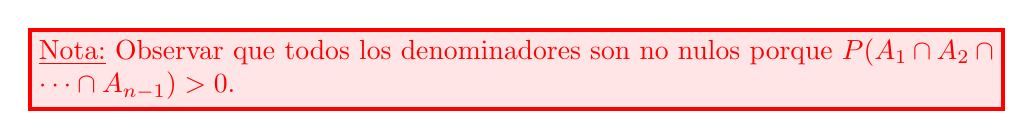
\begin{tikzpicture}
	\node[red, draw=red, fill=red!10, line width=1.5, text width=\textwidth]  {\underline{Nota:} Observar que todos los denominadores son no nulos porque $P(A_1\cap A_2\cap \dots\cap A_{n-1})>0$.};
\end{tikzpicture}

\Ej

Se extraen 3 cartas sin reemplazamiento de la baraja española (40 cartas). Calcular la probabilidad de extraer 3 ases.

$A_i=\text{"Obtengo un As en la $i$-ésima extracción"},\:i=1,2,3$

Me piden $P(A_1\cap A_2\cap A_3)=\lb{\left\{\begin{tabular}{l}
		Teorema de \\
		probabilidad compuesta
\end{tabular}
	\right\}}=\left(\dfrac{4}{40}\right)\cdot\left(\dfrac{3}{39}\right)\cdot\left(\dfrac{2}{38}\right)=\dfrac{1}{2470}$
\begin{itemize}[label=$-$]
	\item Otra forma: \[ \dfrac{\text{casos favorable}}{\text{casos posibles}}=\dfrac{\binom{4}{3}}{\binom{40}{3}}=\dfrac{4}{\frac{40!}{3!37!}}=\dfrac{4}{\frac{40\cdot38\cdot39}{3\cdot 2}}=\dfrac{4\cdot3\cdot2}{40\cdot39\cdot38}=\dfrac{1}{2470} \]
\end{itemize}
\begin{itemize}[label=\color{red}\textbullet, leftmargin=*]
	\item \color{lightblue}Teorema de la Probabilidad Total
\end{itemize}
Sea $(\Omega,\mathcal{S}, P)$ espacio de probabilidad y sean $H_1,H_2,\dots,H_n$ una partición de $\Omega$ con $P(H_i)>0\:\forall i$ y sea $A\in\mathcal{S}$ suceso cualquiera. Entonces: \[ P(A)=P(H_1)\cdot P(A/H_1)+P(H_2)\cdot P(A/H_2)+\cdots +P(H_n)\cdot P(A/H_n). \]
\begin{itemize}[label=\color{red}\textbullet, leftmargin=*]
	\item \color{lightblue}Demostración
\end{itemize}
$A=A\cap\Omega=\lb{\left\{\begin{tabular}{l}
		por ser $(H_1,\dots,H_n)$ partición\\
		de $\Omega$
	\end{tabular}\right\}}=A\cap(H_1\cup H_2\cup \dots \cup H_n)=\lb{\left\{\begin{tabular}{l}
	propiedad\\
	distributiva
	\end{tabular}\right\}}=(A\cap H_1)\cup (A\cap H_2)\cup\dots\cup(A\cap H_n)$

Observar que $(A\cap H_i)$ y $(A\cap H_j)$ son incompatibles o distintos $\forall i\neq j$ por ser $H_i\cap H_j=\varnothing\:\forall i\neq j$.

Tomando probabilidades en la igualdad inicial quedaría \[ P(A)=P(A\cap H_1)+P(A\cap H_2)+\cdots+P(A\cap H_n) \]Regla del Producto $=P(H_1)\cdot P(A/H_1)+P(H_2)\cdot P(A/H_2)+\cdots +P(H_n)\cdot P(A/H_n)$
\begin{itemize}[label=\color{red}\textbullet, leftmargin=*]
	\item \color{lightblue}Teorema (de Bayes)
\end{itemize}
En las condiciones del teorema anterior, se tiene que: \[ \underset{i=1,2,\dots,n}{P(H_i/A)}=\dfrac{P(H_i)\cdot P(A/H_i)}{P(H_1)\cdot P(A/H_1)+P(H_2)\cdot P(A/H_2)+\cdots +P(H_n)\cdot P(A/H_n)} \]
\begin{itemize}[label=\color{red}\textbullet, leftmargin=*]
	\item \color{lightblue}Demostración
\end{itemize}
$ P(H_i/A)=\lb{\left\{\begin{tabular}{l}
		definición probabilidad\\
		condicionada
	\end{tabular}\right\}}=\dfrac{P(A\cap H_i)}{P(A)}=\lb{\left\{\begin{tabular}{l}
	en el numerador aplico la regla del\\
	producto, en el denominador el \\
	Teorema de la Probabilidad Total
	\end{tabular}\right\}}=\dfrac{P(H_i)\cdot P(A/H_i)}{P(H_1)\cdot P(A/H_1)+P(H_2)\cdot P(A/H_2)+\cdots +P(H_n)\cdot P(A/H_n)}$
\begin{itemize}[label=\color{red}\textbullet, leftmargin=*]
	\item \color{lightblue}Nomenclatura
\end{itemize}
$P(H_i)=$ Probabilidad a priori\\
$P(A/H_i)=$ Probabilidad a posteriori

\Ej

Una urna con 3 bolas blancas y 2 negras. Otra urna con 2 bolas blancas y 3 negras. Se lanza un dado y si sale 1 se extrae una bola de la urna 1. En caso, contrario, se extrae de la urna 2.
\begin{enumerate}[label=\color{red}\alph*)]
	\item \lb{Probabilidad de sacar bola blanca.}
	
	$\begin{array}{|c|}
		\begin{array}{l}
			3B\\
			2N
		\end{array}\\ \hline
	\end{array}\qquad\begin{array}{|c|}
	\begin{array}{l}
		2B\\
		3N
	\end{array}\\ \hline
	\end{array}$
	
	$B=$"sacar bola blanca"\\
	$\begin{array}{l}
		U_1=\text{"sacar bola blanca de la urna 1"}\longrightarrow P(U-1)=\dfrac{1}{6}\\
		U_2=\text{"sacar bola blanca de la urna 2"}\longrightarrow P(U_2)=\dfrac{5}{6}
	\end{array}\begin{cases}
	P(B/U_1)=\dfrac{3}{5}\\
	P(B/U_2)=\dfrac{2}{5}
	\end{cases}$
	
	Aplico Teorema de la Probabilidad Total.\\
	$P(B)=P(U_1)\cdot P(B/U_1)+P(U_2)\cdot P(B/U_2)=\dfrac{1}{6}\cdot\dfrac{3}{5}+\dfrac{5}{6}\cdot\dfrac{2}{5}=\dfrac{13}{30}$
	\item \lb{Si sale una bola blanca, probabilidad de que fuera en la urna 1.} \[ P(U_1/B)=\dfrac{P(U_1)\cdot P(B/U_1)}{P(B)}=\dfrac{\frac{1}{6}\cdot\frac{3}{5}}{\frac{13}{30}}=\dfrac{3}{13} \]
	\item \lb{Si sale una bola negra, probabilidad de que fuera en la urna 1.}
	
	$\begin{array}{l}
		P(N)=1-P(B)=1-\dfrac{13}{30}=\dfrac{17}{30}\qquad P(N/U_1)=1-P(B/U_1)=\dfrac{2}{5}\\
		=(U_1/N)=\dfrac{P(U_1)\cdot P(N/U_1)}{P(N)}=\dfrac{\frac{1}{6}\cdot\frac{2}{5}}{\frac{17}{30}}=\dfrac{2}{17}
	\end{array}$
\end{enumerate}
\subsection{Independencia de sucesos}
\begin{itemize}[label=\color{red}\textbullet, leftmargin=*]
	\item \color{lightblue}Definición
\end{itemize}
Sea $(\Omega,\mathcal{S},P)$ un espacio de probabilidad y sean $A,B\in\mathcal{S}$ sucesos. Diremos que $A$ y $B$ son \lb{independientes} si $P(A\cap B)=P(A)\cdot P(B)$

$\bboxed{P(A/B)=\dfrac{P(A\cap B)}{P(B)}\longrightarrow P(A\cap B)=P(B)\cdot P(A/B)=P(A)\cdot P(B/A)}$
\begin{itemize}[label=\color{red}\textbullet, leftmargin=*]
	\item \color{lightblue}Propiedad
\end{itemize}
\begin{enumerate}[label=\color{lightblue}\arabic*)]
	\item $A$ y $B$ son independientes.
	\item $P(A/B)=P(A)$
	\item $P(B/A)=P(B)$
\end{enumerate}
\begin{itemize}[label=\color{red}\textbullet, leftmargin=*]
	\item \color{lightblue}Demostración trivial usando regla de productos:
\end{itemize}
\begin{enumerate}[label=\color{lightblue}\arabic*)]
	\item Si $A$ y $B$ son independientes
	\begin{enumerate}[label=\color{lightblue}1.\arabic*)]
		\item $A$ y $B^c$ son independientes
		\item $A^c$ y $B$ son independientes
		\item $A^c$ y $B^c$ son independientes
	\end{enumerate}
\end{enumerate}
\begin{itemize}[label=\color{red}\textbullet, leftmargin=*]
	\item \color{lightblue}Definición
\end{itemize}
\begin{wrapfigure}[2]{r}{0.5\textwidth}
	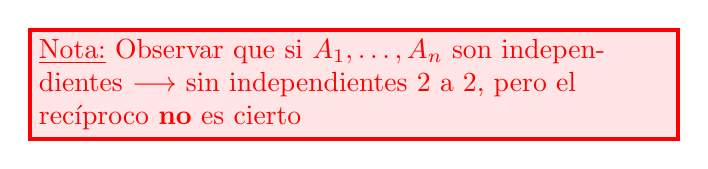
\begin{tikzpicture}
		\node[red, draw=red, fill=red!10, line width=1.5, text width=8cm] {\underline{Nota:} Observar que si $A_1,\dots,A_n$ son independientes $\longrightarrow$ sin independientes 2 a 2, pero el recíproco \textbf{no} es cierto};
	\end{tikzpicture}
\end{wrapfigure}

Diremos que $A_1,\dots,A_n$ son \lb{independientes} si se cumple que: 

$P(\underset{i\in I}{\cap}A)=\underset{i\in I}{\pi}\cdot P(A_i)\quad \forall I\le \{1,2,\dots,n\}$
\begin{itemize}[label=\color{red}\textbullet, leftmargin=*]
	\item \color{lightblue}Teorema (de Bayes generalizado)
\end{itemize}
Sea $(\Omega,\mathcal{S}, P)$ un espacio de probabilidad y sea $\{H_1,\dots, H_n\}$ partición $\Omega$. Sean $A$ y $B\in\mathcal{S}$ con $P(A\cap H_i)>0\:\forall i=1,\dots,n$ \[ P(B/A)=\dfrac{\displaystyle\sum_{i=1}^{n}P(H_i)\cdot P(A/H_i)\cdot P(B/A\cap H_i)}{\displaystyle\sum_{i=1}^{n}P(H_i)\cdot P(A/H_i)} \]
\begin{itemize}[label=\color{red}\textbullet, leftmargin=*]
	\item \color{lightblue}Demostración
\end{itemize}
\begin{center}
	$P(B/A)=\dfrac{P(B\cap A)}{P(A)}$\qquad\begin{minipage}[l]{6cm}
	\lb{Aplico el teorema de la Probabilidad Total tanto a numerado como denominador}
\end{minipage}
\end{center}




\end{document}



